% Báo cáo bài tập lớn INT4418, Nhóm 3. Biên dịch bằng XeLaTeX hoặc Tectonic (xem README.md cùng thư mục).
% Mọi số liệu lấy từ results/figures và results/raw; hình trong figures/ sinh bằng scripts/make_figures.py --report.
\documentclass[11pt,a4paper,oneside]{report}

\usepackage{amsmath}
\usepackage[vietnamese]{babel}
\usepackage{fontspec}
\usepackage{unicode-math}
\setmainfont{texgyretermes}[Extension=.otf,UprightFont=*-regular,BoldFont=*-bold,
  ItalicFont=*-italic,BoldItalicFont=*-bolditalic]
\setmathfont{texgyretermes-math.otf}
\setmonofont{DejaVuSansMono}[Extension=.ttf,BoldFont=*-Bold,Scale=0.8]

\usepackage[a4paper,top=2.2cm,bottom=2.2cm,left=2.5cm,right=2cm]{geometry}
\usepackage{microtype}
\usepackage[table]{xcolor}
\usepackage{graphicx}
\usepackage{booktabs,tabularx,array,multirow}
\usepackage{siunitx}
\usepackage{caption,subcaption}
\usepackage{enumitem}
\usepackage{fancyhdr}
\usepackage{titlesec}
\usepackage{fancyvrb}
\usepackage{float}
\usepackage{etoolbox}
\usepackage{placeins}
\usepackage{needspace}
\AtBeginEnvironment{table}{\small}
\usepackage{tikz}
\usetikzlibrary{arrows.meta,positioning,fit,backgrounds}
\usepackage[hidelinks]{hyperref}
\usepackage{xurl}

\sisetup{output-decimal-marker={,},group-separator={.},group-minimum-digits=4,detect-all}
\captionsetup{font=small,labelfont=bf,labelsep=period,skip=6pt}
\setlist{itemsep=2pt,topsep=4pt}
\renewcommand{\arraystretch}{1.15}
\graphicspath{{figures/}}
\setlength{\parskip}{3pt}
\renewcommand{\topfraction}{0.85}
\renewcommand{\bottomfraction}{0.6}
\renewcommand{\textfraction}{0.12}
\renewcommand{\floatpagefraction}{0.75}
\setlength{\textfloatsep}{12pt plus 2pt minus 4pt}
\setlength{\intextsep}{10pt plus 2pt minus 2pt}
\makeatletter
\setlength{\@fptop}{0pt}
\setlength{\@fpsep}{14pt plus 4pt}
\setlength{\@fpbot}{0pt plus 1fil}
\makeatother
\addto\captionsvietnamese{%
  \renewcommand{\bibname}{Tài liệu tham khảo}%
  \renewcommand{\contentsname}{Mục lục}%
  \renewcommand{\listfigurename}{Danh sách hình vẽ}%
  \renewcommand{\listtablename}{Danh sách bảng}%
  \renewcommand{\chaptername}{Chương}%
  \renewcommand{\appendixname}{Phụ lục}}

% Tiêu đề chương gọn hơn mặc định của lớp report
\titleformat{\chapter}[display]{\normalfont\bfseries}{\large\MakeUppercase{\chaptertitlename}\ \thechapter}{4pt}{\LARGE}
\titlespacing*{\chapter}{0pt}{-12pt}{18pt}

\definecolor{chuthich}{HTML}{52514E}
\definecolor{nhan}{HTML}{2A78D6}
\newcommand{\code}[1]{\texttt{#1}}
% Mục nhóm còn phải điền trước khi nộp; hiển thị màu đỏ để không bị bỏ sót.
\newcommand{\canchot}[1]{\textcolor{red!70!black}{[#1]}}

\pagestyle{fancy}
\fancyhf{}
\fancyhead[L]{\small\nouppercase{\leftmark}}
\fancyhead[R]{\small INT4418 Dữ liệu lớn}
\fancyfoot[C]{\small \thepage}
\renewcommand{\headrulewidth}{0.4pt}
\renewcommand{\chaptermark}[1]{\markboth{\chaptertitlename\ \thechapter. #1}{}}
\fancypagestyle{plain}{\fancyhf{}\fancyfoot[C]{\small \thepage}\renewcommand{\headrulewidth}{0pt}}

\begin{document}

% ---------------------------------------------------------------- Trang bìa
% Đặt tuyệt đối theo trang (đơn vị bp, gốc ở góc trên trái) để khung viền và logo khớp mẫu bìa của Học viện.
\begin{titlepage}
\begin{tikzpicture}[remember picture,overlay]
\begin{scope}[shift={(current page.north west)},x=1bp,y=-1bp,every node/.style={inner sep=0pt}]
\node[anchor=north west] at (49.5,31.45) {
\includegraphics[width=499.35bp,height=762.75bp]{assets/khung_bia.jpg}};
\draw[blue,line width=0.75bp] (49.2,31.2) rectangle (549.2,794.6);
\node[anchor=base] at (297.64,85.5) {\fontsize{14}{16}\selectfont\bfseries HỌC VIỆN CÔNG NGHỆ BƯU CHÍNH VIỄN THÔNG};
\node[anchor=base] at (297.64,100.6) {\fontsize{13}{15}\selectfont\bfseries KHOA ĐÀO TẠO SAU ĐẠI HỌC};
\node[anchor=north west] at (246.55,119) {
\includegraphics[width=102.2bp,height=132.8bp]{assets/logo_ptit.png}};
\draw[line width=1.8bp] (232.8,121.3) -- (360,121.3);
\node[anchor=base] at (297.64,340.8) {\fontsize{20}{24}\selectfont\bfseries BÁO CÁO BÀI TẬP LỚN DỮ LIỆU LỚN};
\node[anchor=base] at (297.64,380) {\fontsize{18}{22}\selectfont\bfseries Lean Premise Retrieval: Truy hồi thưa và truy hồi};
\node[anchor=base] at (297.64,404) {\fontsize{18}{22}\selectfont\bfseries lai trên mathlib4};
\node[anchor=base] at (297.64,423.6) {\fontsize{13}{15}\selectfont\itshape Truy hồi định lý/bổ đề bằng từ khóa, ký hiệu và đặc trưng cấu trúc};
\begin{scope}[every node/.append style={anchor=base west,font=\fontsize{13}{15}\selectfont\bfseries}]
\node at (112,492.6) {Giảng viên hướng dẫn:}; \node at (251,492.6) {TS. NGUYỄN KIỀU LINH};
\node at (112,511.6) {Lớp:};                  \node at (251,511.6) {M25CQHT02-B};
\node at (112,530.6) {Mã nhóm:};              \node at (251,530.6) {3};
\node at (112,549.6) {Thành viên:};
\end{scope}
\foreach \ten/\ma [count=\i from 0] in {NGUYỄN ĐỨC HOÀNG/B25CHHT096,NGUYỄN MẠNH CƯỜNG/B25CHHT082,
    TRẦN DUY KHÁNH/B25CHHT100,TRẦN ĐÌNH DŨNG/B25CHHT089,VŨ TRUNG KIÊN/B25CHHT101,NGUYỄN NGỌC MINH/B25CHHT106}{
  \node[anchor=base west,font=\fontsize{11}{13}\selectfont\bfseries] at (251,549.6+16.4*\i) {\ten};
  \node[anchor=base west,font=\fontsize{11}{13}\selectfont\bfseries] at (389,549.6+16.4*\i) {- \ma};
}
\node[anchor=base] at (297.64,719.6) {\fontsize{13}{15}\selectfont\bfseries\itshape Hà Nội – 2026};
\end{scope}
\end{tikzpicture}
\end{titlepage}

% ---------------------------------------------------------------- Phần đầu
\pagenumbering{roman}
\chapter*{Tóm tắt}
\phantomsection\addcontentsline{toc}{chapter}{Tóm tắt}
\markboth{Tóm tắt}{}
\noindent
Báo cáo trình bày một hệ thống premise retrieval cho Lean 4 trên thư viện mathlib4, kết hợp BM25F với các đặc trưng
cấu trúc có chi phí tính toán thấp. Dữ liệu là LeanDojo Benchmark 4 bản v10 với \num{180957} khai báo; sau khi lọc, tập
test của split \code{random} còn \num{2641} truy vấn, mỗi truy vấn là một proof state. Chỉ mục đảo được xây theo mô hình
MapReduce trên Apache Spark và bằng một chương trình tuần tự; hai cách cho kết quả trùng từng byte. Ở cấu hình V4, BM25F
dùng tokenizer riêng cho Lean trên ba trường name, namespace và statement, bộ lọc chỉ giữ accessible premise, tức premise có thể
dùng tại vị trí chứng minh hiện tại, rồi hồi quy logistic rerank 100 candidate bằng đặc trưng cấu trúc,
popularity và PageRank. Trên tập test \code{random}, Recall@10 tăng từ 0,100 của BM25 mặc định lên 0,243. V5 bổ sung
candidate từ lịch sử sử dụng trong tập train, đạt 0,281 trên tập test và 0,332 so với 0,310 của V4 trên holdout lấy từ
phần train chưa dùng để huấn luyện reranker. Tuy vậy, trên holdout chưa có đủ bằng chứng cho thấy V5 tốt hơn đối chứng V4
lấy top 240 candidate, và trên tập test \code{novel\_premises}, Recall@10 trên unseen premise giảm từ 0,444 xuống 0,359.
Trong cùng một phiên đo tải, P95 latency ở 10 client của V4 và V5 là 103,2 và 116,7 ms; ở 50 client, thông lượng của V5
giảm từ 132 xuống 116 truy vấn mỗi giây. Dịch vụ bị giới hạn bởi CPU, và Spark local[8] nhanh hơn bản tuần tự 3,84 lần
trên corpus nhân bản 3,6 triệu bản ghi. Mọi phép đo thực hiện trên một máy; so sánh với hệ thống dense retrieval của
Nhóm 4 chưa hoàn tất.

\medskip\noindent
\textbf{Từ khóa:} premise retrieval, Lean 4, mathlib4, BM25F, chỉ mục đảo, MapReduce, Apache Spark.

\setcounter{tocdepth}{1}
\tableofcontents
\clearpage\phantomsection\addcontentsline{toc}{chapter}{\listfigurename}
\listoffigures
\begingroup\let\clearpage\relax\let\cleardoublepage\relax
\vspace{1.5cm}\phantomsection\addcontentsline{toc}{chapter}{\listtablename}
\listoftables
\endgroup
\clearpage
\pagenumbering{arabic}

% ================================================================ 1
\chapter{Giới thiệu}

Lean 4 là một trợ lý chứng minh đồng thời là ngôn ngữ lập trình~\cite{demoura2021}, và mathlib4 là thư viện toán học
lớn nhất viết bằng Lean~\cite{mathlib2020}. Khi chứng minh một định lý mới, người dùng hoặc bộ chứng minh tự động phải
chọn trong thư viện những định lý, bổ đề và định nghĩa có thể dùng ở bước tiếp theo. Các đối tượng này được gọi là
\emph{premise}. Bài toán \emph{premise retrieval} được phát biểu như sau: cho proof state (trạng thái chứng minh) hiện
tại, trả về một danh sách ngắn các premise có khả năng được dùng trong tactic kế tiếp~\cite{yang2023}. Chất lượng của danh
sách này ảnh hưởng trực tiếp tới khả năng thành công của bộ chứng minh, vì bộ chứng minh không thể xét toàn bộ thư viện ở
mỗi bước. Có hai hướng tiếp cận chính: sparse retrieval so khớp từ khóa trên chỉ mục đảo, điển hình là BM25; dense
retrieval mã hóa truy vấn và premise thành vector bằng mô hình neural rồi tìm láng giềng gần nhất; hybrid retrieval kết
hợp cả hai. Báo cáo này thuộc hướng sparse retrieval, có bổ sung đặc trưng cấu trúc.

Bài toán có ba đặc điểm của dữ liệu lớn. Thứ nhất là khối lượng: snapshot mathlib4 được dùng có \num{180957} khai báo,
và mỗi bước chứng minh sinh ra một truy vấn, nên nếu so khớp từng truy vấn với mọi khai báo thì chi phí tăng tuyến tính
theo kích thước kho và theo số truy vấn cần phục vụ. Thứ hai là phân bố lệch: từ khóa \code{theorem} xuất hiện trong
\num{109826} phát biểu, ký hiệu \code{=} trong hơn \num{80000} phát biểu. Các token này tạo ra khóa nóng (hot key) ở pha
shuffle khi xây chỉ mục và posting list dài khi truy vấn. Thứ ba là yêu cầu phục vụ: hệ thống phải trả lời nhiều truy vấn
đồng thời và giữ P95 latency ở mức thấp, đồng thời chỉ mục phải xây lại được khi thư viện đổi phiên bản.

Nhóm đặt hai câu hỏi nghiên cứu theo đề bài:
\begin{enumerate}[label=\textbf{RQ\arabic*.},leftmargin=*]
  \item BM25 có đủ mạnh cho dữ liệu Lean, hay cần bổ sung trường ký hiệu, namespace và thông tin phụ thuộc?
  \item Kết hợp điểm BM25F với các đặc trưng cấu trúc có làm tăng Recall@$k$ mà vẫn giữ được P95 latency thấp hay không?
\end{enumerate}
Hai câu hỏi cùng hướng tới câu hỏi trung tâm của đề: đặc trưng cấu trúc thực sự cải thiện recall hay chỉ làm tăng chi
phí. Nhóm chọn hai chỉ số chính là Recall@10 cho chất lượng và P95 latency ở 10 client đồng thời cho chi phí; các chỉ số
khác dùng để giải thích đánh đổi.

Đóng góp của nhóm gồm bốn phần:
\begin{enumerate}[leftmargin=*]
  \item Một đặc tả benchmark và pipeline trích xuất tái lập được từ LeanDojo Benchmark 4, có data contract, bảng
        dead-letter cho mọi bản ghi bị loại, thống kê luồng lọc theo từng tập và kiểm tra tự động 20 truy vấn mẫu.
  \item Một chỉ mục đảo xây theo mô hình MapReduce bằng hai engine Spark, trùng từng byte với bản tuần tự, cùng thí
        nghiệm xây chỉ mục tới 3,6 triệu bản ghi (corpus nhân bản) trên Windows và Linux của cùng một máy, có đo
        shuffle, bộ nhớ, độ lệch và nén.
  \item Một hệ thống truy hồi hai giai đoạn gồm BM25F và reranker cấu trúc (V4), cùng biến thể V5 bổ sung candidate từ
        lịch sử sử dụng trong tập train, được đối chiếu với V4 lấy top 240 candidate và kiểm tra trên một holdout chưa
        dùng để huấn luyện hay chọn cấu hình.
  \item Một bộ đánh giá gồm chất lượng và độ trễ trên ba kích thước chỉ mục và ba mức tải, khoảng tin cậy bootstrap
        theo cụm theorem và kiểm định hoán vị theo cụm có hiệu chỉnh Holm, ablation, phân rã giới hạn giữa bước tạo
        candidate và bước xếp hạng, và phân tích lỗi.
\end{enumerate}

Phần còn lại của báo cáo được tổ chức như sau. Chương~\ref{sec:related} điểm qua công trình liên quan.
Chương~\ref{sec:data} mô tả dữ liệu và định nghĩa benchmark. Chương~\ref{sec:method} trình bày kiến trúc và thuật toán.
Chương~\ref{sec:setup} nêu thiết lập thí nghiệm, Chương~\ref{sec:results} trình bày kết quả, Chương~\ref{sec:ablation}
trình bày ablation, phân tích lỗi, hạn chế và threats to validity. Chương~\ref{sec:conclusion} kết luận.

% ================================================================ 2
\chapter{Công trình liên quan}\label{sec:related}

\paragraph{Sparse retrieval.} BM25 và mở rộng nhiều trường BM25F được Robertson và Zaragoza tổng kết trong khung xác
suất về độ liên quan~\cite{robertson2009}. BM25F chuẩn hóa tần suất của từng trường theo độ dài trường rồi mới áp dụng
hàm bão hòa, nên một term xuất hiện ở nhiều trường không bị tính quá mức như khi cộng điểm BM25 của từng trường. Cấu trúc
chỉ mục đảo (inverted index), mã hóa khoảng cách (d-gap), mã Variable-byte và mã gamma được trình bày trong giáo trình của
Manning và cộng sự~\cite{manning2008}; Scholer và cộng sự chỉ ra rằng mã theo byte giải mã nhanh hơn đáng kể so với mã
theo bit với tỉ lệ nén chấp nhận được~\cite{scholer2002}. Hệ thống của nhóm dùng BM25F làm giai đoạn đầu và đo lại đánh
đổi nén trên dữ liệu Lean.

\paragraph{Chọn premise trong trợ lý chứng minh.} MePo, bộ lọc liên quan dùng trong Sledgehammer của Isabelle, chọn
premise theo mức trùng ký hiệu với mục tiêu và mở rộng dần theo các ký hiệu mới~\cite{meng2009}. DeepMath dùng mô hình
chuỗi học sâu để chọn premise cho thư viện Mizar~\cite{irving2016}. Magnushammer học biểu diễn bằng transformer theo
phương pháp tương phản và vượt Sledgehammer trên Isabelle~\cite{mikula2024}. LeanDojo xây công cụ trích xuất dữ liệu từ
Lean, giới thiệu LeanDojo Benchmark với hai split \code{random} và \code{novel\_premises}, đồng thời đề xuất ReProver, một
hệ thống chứng minh kết hợp mô hình sinh tactic với dense retriever; thành phần retrieval chỉ tìm trong các accessible
premise, tức premise có thể dùng tại vị trí đang chứng minh~\cite{yang2023,leandojodocs}.
Nhóm dùng lại benchmark và ý tưởng accessible premise, nhưng giữ toàn bộ hệ thống ở dạng sparse retrieval và không dùng
mô hình neural; hướng dense retrieval do Nhóm 4 của lớp khảo sát.

\paragraph{Xây chỉ mục phân tán.} MapReduce~\cite{dean2004} và Spark với mô hình RDD~\cite{zaharia2012,sparkdocs} là
hai mô hình tính toán phổ biến để xây chỉ mục đảo theo lô. Lin và Dyer mô tả các mẫu thiết kế cho bài toán này, trong
đó có kết hợp cục bộ trong mapper và chuyển giá trị thành một phần của khóa để reducer nhận dữ liệu đã sắp
xếp~\cite{lin2010}. Hệ thống của nhóm cài đặt các mẫu này trên Spark và đo tác động của chúng.

\paragraph{Tín hiệu đồ thị và trộn xếp hạng.} PageRank~\cite{page1999} được dùng trên đồ thị theorem tới premise để ước
lượng mức quan trọng của premise. Reciprocal Rank Fusion~\cite{cormack2009} trộn hai danh sách xếp hạng mà không cần
chuẩn hóa điểm, phù hợp để kết hợp hệ thống sparse retrieval của Nhóm 3 với hệ thống dense retrieval của Nhóm 4 thành
hybrid retrieval.

\paragraph{Khoảng trống.} Các hệ thống premise retrieval gần đây chủ yếu dùng dense retrieval và báo cáo chất lượng
trên một cấu hình phần cứng cố định. Ít công trình đo riêng xem BM25F cộng các đặc trưng cấu trúc có chi phí tính toán thấp đạt tới mức nào, và
chi phí xây chỉ mục cùng độ trễ thay đổi ra sao khi kho tăng. Báo cáo này tập trung vào khoảng trống đó.

% ================================================================ 3
\chapter{Dữ liệu}\label{sec:data}

\section{Nguồn, phiên bản và lược đồ}

Dữ liệu là LeanDojo Benchmark 4 bản v10 (Bảng~\ref{tab:source} ở Phụ lục~\ref{app:tables}), tải từ
Zenodo~\cite{zenodo2024} và kiểm tra md5 trước khi giải nén; script ghi manifest gồm đường dẫn, kích thước và mã băm. Dữ
liệu đầy đủ không được đưa vào Git; kho mã chỉ chứa mẫu gồm \num{1000} premise và 200 truy vấn cùng script tải và tạo lại
dữ liệu. Pipeline trích xuất chuyển JSON sang năm bảng Parquet (Bảng~\ref{tab:schema}). Mỗi premise được định danh bằng cặp
(\code{full\_name}, \code{path}) vì có 57 tên xuất hiện đồng thời trong Lean core và Mathlib, ví dụ \code{not\_le}; mã
\code{premise\_id} là thứ tự của cặp này nên ổn định với cùng snapshot. Trường \code{statement} là mã nguồn cắt tại dấu
\code{:=} ở cấp ngoài cùng, tại \code{where} hoặc tại nhánh \code{|} đầu dòng, để không đưa phần chứng minh vào chỉ mục;
mô tả từng cột nằm trong \code{docs/data\_dictionary.md}. Corpus gồm \num{156947} khai báo của Mathlib, \num{19619} của Lean
core, \num{2883} của Batteries và phần nhỏ của các thư viện khác; theo loại có \num{109823} \code{theorem}, \num{36826}
\code{def}, \num{16969} \code{lemma} và \num{10071} \code{instance}.

\section{Truy vấn và gold premise}

Một truy vấn là trường \code{state\_before} của một tactic có ít nhất một premise được chú thích; tập gold premise là
các premise trong chú thích đó. Văn bản của tactic không được đưa vào truy vấn vì nó chứa sẵn tên premise cần tìm. Ví dụ,
trong truy vấn \code{random:val:36:0}, mục tiêu là chứng minh tích của \code{a}, nghịch đảo của \code{b} và \code{b} bằng
\code{a} trong một monoid; tactic \code{simp [mul\_assoc]} dùng premise \code{mul\_assoc}, còn hệ thống chỉ được thấy proof
state. Truy vấn này là truy vấn đầu tiên trong mẫu 20 truy vấn kiểm tra (\code{docs/check\_queries.md}) và được dùng làm ví dụ xuyên suốt
(Bảng~\ref{tab:example}). Ngoài proof state, hệ thống được dùng tên theorem đang chứng minh, tệp chứa nó và dòng bắt đầu
của nó; bộ lọc accessible premise luôn loại chính theorem này ra.

Có \num{115736} lượt gold premise không có trong corpus và bị loại. Hiện tượng này đến từ bản thân benchmark: các bổ đề sinh
tự động bởi \code{@[to\_additive]} như \code{add\_comm}, các constructor như \code{Or.inl} và các trường của structure như
\code{Iff.mp} không phải khai báo tường minh trong \code{corpus.jsonl}. Sau khi loại, \num{20544} truy vấn không còn gold
premise nào và cũng bị loại; mọi bản ghi bị loại được ghi vào bảng \code{dead\_letter} kèm lý do. Vì vậy recall báo cáo chỉ
tính premise có trong corpus và cao hơn recall mà bộ chứng minh gặp thực tế.

\section{Split và tập đánh giá}

Nhóm giữ nguyên hai split của LeanDojo. Split \code{random} là split chính; split \code{novel\_premises} được thiết kế
để khó hơn: mỗi chứng minh trong tập test dùng ít nhất một premise chưa từng được dùng trong tập train. Mọi tham
số chỉ được chọn trên validation. Bảng~\ref{tab:dataflow} theo dõi số lượng qua từng bước lọc. Mỗi split có \num{2000}
theorem trong tập test, nhưng chỉ 882 theorem của \code{random} và \num{1196} theorem của \code{novel\_premises} còn ít nhất một
truy vấn, tức 44,1\% và 59,8\%. Nguyên nhân chính là khoảng một nửa số theorem được chứng minh trực tiếp bằng term nên
không có tactic nào. Kết quả chất lượng vì vậy đại diện cho các chứng minh dạng tactic có chú thích premise, không phải
cho mọi theorem. Con số \num{315014} của bảng \code{queries} là tổng lượt truy vấn của cả hai split; trong từng tập, số
proof state khác nhau ít hơn số truy vấn chưa tới 1\%.

\input{tables/dataflow}

\paragraph{Tính chất novel sau khi lọc.} Bảo đảm của split \code{novel\_premises} đặt ở cấp chứng minh, còn đánh giá
diễn ra ở cấp tactic sau khi lọc nhãn. Gọi một gold premise là unseen premise nếu nó không xuất hiện trong nhãn của
tập train cùng split (khác với premise vắng khỏi corpus), ngược lại là seen premise. Chỉ \num{2506} trên \num{9735} cặp
(truy vấn, gold premise) của tập test, tức 25,7\%, là unseen premise, gồm \num{1933} premise khác nhau; 103 trên
\num{1196} theorem được chấm không còn unseen premise nào. Recall tổng thể của split này vì vậy chủ yếu là recall trên
seen premise; Mục~\ref{sec:robust} báo cáo riêng recall trên unseen premise.

Tập train được chia đôi cố định theo md5 của tên theorem: train A dùng để tính thống kê phụ thuộc như popularity và
PageRank, train B dùng để huấn luyện reranker, để đặc trưng không chứa nhãn của chính truy vấn dùng để huấn luyện. Thống kê và mô
hình cho \code{novel\_premises} được tính lại từ tập train của split này, vì tập train của \code{random} chứa các
theorem thuộc tập test của \code{novel\_premises}.

\paragraph{Tập con cho thí nghiệm quy mô.} Nhóm lấy mẫu 500 truy vấn trong tập test \code{random} (seed 42) và tạo ba chỉ mục
lồng nhau 10K, 100K và 181K premise, đều chứa 870 gold premise của mẫu, phần còn lại lấy ngẫu nhiên. Thí nghiệm xây
chỉ mục dùng thêm hai corpus nhân bản nội dung gấp 5 lần (\num{904785} bản ghi) và gấp 20 lần (\num{3619140} bản ghi), chỉ
để đo thời gian, bộ nhớ và độ lệch.

% Tạm ẩn Mục 3.4 cho đến khi đối chiếu thủ công xong 20 truy vấn kiểm tra.
% \section{Kiểm tra chất lượng dữ liệu}\label{sec:checkdata}
%
% Script \code{make\_check\_queries.py} lấy 20 truy vấn validation (seed 42, mỗi lĩnh vực nhiều nhất hai truy vấn) và kiểm
% tra tự động bốn điều kiện so với tactic gốc: gold premise được đánh dấu trong tactic, là accessible premise của theorem, không
% phải chính theorem, và mọi premise bị loại đều có trong dead-letter. Cả 20 truy vấn đạt bốn điều kiện; 16 bản ghi trùng hoàn toàn
% đã được loại. Bước đối chiếu thủ công từng truy vấn và ký xác nhận trong \code{docs/check\_queries.md} chưa được thực hiện.

% ================================================================ 4
\chapter{Phương pháp và kiến trúc}\label{sec:method}

\section{Tổng quan}

Hệ thống gồm hai đường xử lý (Hình~\ref{fig:arch}). Đường xây chỉ mục chạy theo lô: trích xuất dữ liệu, tokenize và
xây chỉ mục đảo theo mô hình MapReduce. Đường phục vụ chạy trực tuyến: nhận proof state cùng ngữ cảnh, tokenize bằng đúng
tokenizer và phiên bản đã dùng khi xây chỉ mục, dùng BM25F trên ba trường name, namespace và statement để lấy top 100
accessible premise làm candidate, rồi reranker dùng hồi quy logistic để xếp hạng lại dựa trên các đặc trưng cấu trúc,
popularity và PageRank (V4). V5 bổ sung candidate từ lịch sử sử dụng trong train A và thêm hai đặc trưng
\code{file\_usage}, \code{dir\_usage}.

\begin{figure}[htbp]
\centering
\begin{tikzpicture}[
  node distance=3.2mm and 7mm,
  khoi/.style={draw=chuthich,rounded corners=2pt,fill=white,align=center,font=\small,minimum width=5.0cm,minimum height=7mm,inner sep=2pt},
  phu/.style={khoi,font=\small,minimum width=4.0cm,text width=3.8cm},
  dl/.style={khoi,fill=nhan!8},
  mui/.style={-{Stealth[length=2.2mm]},thick,draw=chuthich}]
  \node[dl] (raw) {LeanDojo Benchmark 4 v10\\(corpus.jsonl, train/val/test.json)};
  \node[khoi,below=of raw] (ext) {Trích xuất theo data contract\\premises, queries, qrels, files, dead-letter};
  \node[khoi,below=of ext] (map) {Map: tách từ, đếm cục bộ\\phát ((field, term), (doc\_id, tf))};
  \node[khoi,below=of map] (shuf) {Shuffle: hash(field, term) mod R\\tách khóa nóng theo khoảng doc\_id};
  \node[khoi,below=of shuf] (red) {Reduce: sắp posting theo doc\_id\\mã d-gap và Variable-byte};
  \node[dl,below=of red] (idx) {Chỉ mục đảo: dictionary, postings.bin\\manifest có SHA-1 từng tệp};
  \node[dl,right=of raw] (q) {Proof state và ngữ cảnh\\(theorem, tệp, dòng bắt đầu)};
  \node[khoi,below=of q] (tok) {Tách từ Lean (cùng phiên bản)};
  \node[khoi,below=of tok] (s1) {Giai đoạn 1: BM25F trên 3 trường\\lọc accessible premise, top 100};
  \node[khoi,below=of s1] (mg) {Hợp nhất, loại trùng: 100 candidate;\\V5 thêm tối đa 250, tổng trung bình 239};
  \node[khoi,below=of mg] (s2) {Giai đoạn 2: hồi quy logistic\\13 đặc trưng (V4) hoặc 15 (V5)};
  \node[dl,below=of s2] (out) {Top-$k$ premise qua FastAPI hoặc CLI};
  \node[phu,right=of mg] (ex) {Chỉ ở V5: premise dùng nhiều nhất ở cùng tệp (100), cùng thư mục (100), toàn thư viện (50)};
  \node[phu,right=of out] (dep) {Thống kê từ train A: popularity, PageRank (tĩnh); số lần dùng theo tệp, thư mục (theorem có trước)};
  \draw[mui] (raw) -- (ext); \draw[mui] (ext) -- (map); \draw[mui] (map) -- (shuf);
  \draw[mui] (shuf) -- (red); \draw[mui] (red) -- (idx);
  \draw[mui] (q) -- (tok); \draw[mui] (tok) -- (s1); \draw[mui] (s1) -- (mg); \draw[mui] (mg) -- (s2); \draw[mui] (s2) -- (out);
  \draw[mui] (idx.east) -| ([xshift=-4.5mm]s1.west) -- (s1.west);
  \draw[mui] (ex) -- (mg);
  \draw[mui] (dep.north) -- (ex.south);
  \draw[mui] (dep.west) -| ([xshift=4.5mm]s2.east) -- (s2.east);
  \begin{scope}[on background layer]
    \node[fit=(raw)(idx),draw=chuthich!50,dashed,rounded corners=4pt,inner sep=4pt,label={[font=\small\bfseries]above:Đường xây chỉ mục (theo lô)}] {};
    \node[fit=(q)(out)(ex)(dep),draw=chuthich!50,dashed,rounded corners=4pt,inner sep=4pt,label={[font=\small\bfseries]above:Đường phục vụ (trực tuyến)}] {};
  \end{scope}
\end{tikzpicture}
\caption[Kiến trúc hệ thống]{Kiến trúc hệ thống. Bản xây chỉ mục tuần tự và bản Spark cho cùng một chỉ mục. Candidate bổ
sung của V5 cũng qua bộ lọc accessible premise; 239 là tổng số candidate trung bình của V5 trên tập test \code{random}, gồm
cả 100 candidate của BM25F.}\label{fig:arch}
\end{figure}

\section{Tokenizer cho Lean}

Tokenizer mặc định của baseline chỉ lấy các chuỗi chữ và số rồi chuyển về chữ thường, nên làm mất ký hiệu toán học và
tên ghép. Tokenizer Lean giữ tên đầy đủ có dấu chấm đồng thời tách thành các thành phần, ví dụ \code{Nat.add\_comm} sinh
ra \code{nat.add\_comm}, \code{nat}, \code{add\_comm}, \code{add} và \code{comm}; tách thêm theo camelCase (\code{natAbs}
thành \code{nat} và \code{abs}); giữ các ký hiệu như $\forall$, $\to$, $\le$, $\neq$, $\mathbb{N}$, $\mathbb{R}$ làm token;
và bỏ biến một chữ cái ASCII. Tokenizer không dùng chuẩn hóa NFKC vì NFKC biến $\mathbb{R}$ thành chữ R thường. Phiên bản
tokenizer được ghi trong manifest của chỉ mục để đường phục vụ dùng đúng phiên bản.

\section{Xây chỉ mục theo mô hình MapReduce}\label{sec:mapreduce}

Đơn vị dữ liệu là một premise với ba trường \code{name}, \code{namespace} và \code{statement}. Nhóm cài đặt hai engine Spark
cho cùng một đầu ra; engine thứ hai được viết lại sau khi đo engine thứ nhất (Mục~\ref{sec:engines}).

\paragraph{Engine RDD.} Driver đọc dữ liệu rồi phân phối cho các executor. Mapper phân tích văn bản, đếm tần suất của term
trong tài liệu ngay tại chỗ (kết hợp cục bộ) rồi phát cặp ((field, term), (doc\_id, tf)). Pha shuffle chia dữ liệu theo
$\mathrm{hash}(\text{field}, \text{term}) \bmod R$; khóa nóng có tần suất tài liệu vượt \num{20000} được tách thành $S$ phần
theo khoảng $\lfloor \text{doc\_id} \cdot S / N \rfloor$, nên các phần nối lại theo thứ tự mà không phải sắp xếp lại.
Reducer sắp posting theo doc\_id, tính tần suất, mã hóa và ghi tệp con; driver trộn từ điển theo thứ tự (field, term) cố
định và ghi manifest chứa tham số, thống kê và mã SHA-1 của từng tệp. Nhờ thứ tự cố định, bản Spark và bản tuần tự cho chỉ
mục trùng nhau từng byte, được kiểm tra bằng cách so mã băm.

\paragraph{Engine Arrow.} Engine này giữ nguyên đầu ra nhưng thay đổi ba điểm. Thứ nhất, executor tự đọc Parquet qua Spark
SQL; driver chỉ đọc cột \code{premise\_id} để đánh doc\_id, nên bộ nhớ của driver không tăng theo nội dung corpus. Thứ hai,
mã Python nhận dữ liệu theo lô Arrow (\code{mapInArrow}) và gộp posting ở mức partition: mỗi partition phát một bản ghi cho
mỗi cặp (field, term) nó chứa, mang cả dãy doc\_id và dãy tf dưới dạng mảng nhị phân. Đây là mẫu kết hợp trong mapper của
Lin và Dyer~\cite{lin2010} áp dụng cho cả partition. Thứ ba, shuffle và sắp xếp chạy trong JVM, tần suất tài liệu và độ dài
trường đi kèm dưới dạng khóa đặc biệt, nên chỉ còn một lượt shuffle dữ liệu chính thay vì hai.

Mỗi posting list lưu dãy khoảng cách doc\_id (d-gap) và dãy tf, mã bằng số nguyên 32 bit, Variable-byte (VB, mặc định) hoặc
gamma; ví dụ của giáo trình~\cite{manning2008} (dãy 3, 7, 1, 119 mã VB thành \code{83 87 81 F7}, mã gamma thành 22 bit) nằm
trong unit test. Gọi $T$ là tổng số token, $P$ là số posting, $K$ là số cặp (field, term) và $R$ là số partition. Pha map
tốn $O(T)$. Kết hợp cục bộ của engine RDD giảm số bản ghi shuffle từ $T$ xuống $P$; với engine Arrow, số bản ghi shuffle
không vượt quá $\min(P, K \cdot R)$, còn tổng dung lượng vẫn là $O(P)$. Khi corpus lớn lên, $P$ tăng theo số tài liệu còn
$K$ tăng chậm hơn; với corpus nhân bản ở Chương~\ref{sec:results}, $K$ không đổi nên đây là trường hợp thuận lợi nhất cho
engine Arrow. Pha reduce sắp xếp tổng cộng không quá $O(P \log P_{\max})$. Với chỉ mục ba trường của corpus đầy đủ,
$P = \num{4323308}$ và $K = \num{481002}$.

\section{Hàm xếp hạng BM25 và BM25F}

Với truy vấn $q$ và tài liệu $d$, BM25F tính tần suất đã chuẩn hóa của term $t$ và điểm của tài liệu là
\begin{equation}
\tilde{tf}(t,d) = \sum_{f} w_f \cdot \frac{tf_f(t,d)}{1 - b_f + b_f \cdot \ell_f(d)/\bar{\ell}_f},
\qquad
s(q,d) = \sum_{t \in q} \mathrm{qtf}(t) \cdot \mathrm{idf}(t) \cdot \frac{\tilde{tf}(t,d)\,(k_1 + 1)}{\tilde{tf}(t,d) + k_1},
\end{equation}
trong đó $w_f$ là trọng số trường $f$, $b_f$ là hệ số chuẩn hóa độ dài, $\ell_f(d)$ là độ dài trường, $\bar{\ell}_f$ là độ
dài trung bình và $\mathrm{idf}(t) = \ln\big(1 + (N - \mathrm{df}(t) + 0{,}5)/(\mathrm{df}(t) + 0{,}5)\big)$ không âm như
trong Lucene. Khi chỉ có một trường và $w = 1$, công thức trở về BM25. Hệ số $\mathrm{qtf}(t)$ là số lần term xuất hiện
trong truy vấn hoặc bằng 1 (chế độ nhị phân, phù hợp với proof state nơi tên giả thiết lặp lại nhiều lần). Chi phí của một
truy vấn phụ thuộc vào tổng độ dài các posting list được đọc, $\sum_{t \in q}\sum_f \mathrm{df}_f(t)$, cộng với thao tác gộp
điểm. Cách làm này tránh tính điểm riêng cho từng tài liệu nhưng không độc lập với kích thước kho: posting list của các token phổ
biến như \code{=} hay $\to$ dài ra tuyến tính theo số tài liệu $N$. Cài đặt hiện tại gộp điểm bằng \code{np.unique}, nên có
thêm chi phí sắp xếp $O(M \log M)$ với $M$ là số posting được đọc, và bộ lọc accessible premise tạo mặt nạ trên toàn bộ $N$
premise.

\section{Bộ lọc accessible premise}

Một premise là accessible premise của theorem đang chứng minh nếu nó nằm trong tệp được import trực tiếp hoặc gián tiếp
bởi tệp chứa theorem, hoặc nằm trong cùng tệp và đã khai báo xong trước theorem; chỉ những premise này mới dùng được tại
vị trí chứng minh. Hệ thống tính bao đóng import trên \num{5674} tệp, lưu đệm theo tệp
rồi tạo mặt nạ trên toàn bộ premise. Với premise cùng tệp, điều kiện là dòng \emph{kết thúc} của premise nhỏ hơn dòng bắt
đầu của theorem (Mục~\ref{sec:bug} giải thích lý do). Bộ lọc được áp dụng ở giai đoạn 1, trước khi chọn 100 candidate.

\section{Reranker cấu trúc}

Giai đoạn 2 rerank 100 candidate bằng hồi quy logistic trên 13 đặc trưng ở Bảng~\ref{tab:features}. Đặc trưng chỉ dùng
proof state, ngữ cảnh của truy vấn và thống kê tính trên train A, không dùng nhãn của validation hay tập
test. Mô hình được huấn luyện trên \num{6000} truy vấn lấy ngẫu nhiên từ train B, gồm \num{600000} cặp (truy vấn, candidate) với \num{4492} cặp dương; candidate lúc huấn luyện được sinh bằng đúng giai đoạn 1 và bộ lọc như lúc chạy. Đặc trưng
được chuẩn hóa theo tập train; hệ số điều chuẩn $C = 1$. Đồ thị phụ thuộc có cạnh từ mỗi theorem của train A tới các
premise nó dùng, gồm \num{129983} cạnh và \num{41703} premise; PageRank dùng hệ số damping 0,85 và hội tụ sau 11 vòng lặp.

\begin{table}[htbp]
\centering
\caption[Đặc trưng của reranker]{Đặc trưng của reranker. V3 dùng 11 đặc trưng đầu, V4 dùng 13, V5 dùng đủ 15}\label{tab:features}
\begin{tabularx}{\linewidth}{@{}>{\raggedright\arraybackslash}p{2.1cm}>{\raggedright\arraybackslash}p{3.3cm}X@{}}
\toprule
Nhóm & Đặc trưng & Ý nghĩa \\
\midrule
Điểm giai đoạn 1 & \code{bm25\_rel}, \code{bm25\_rr} & điểm BM25F chia cho điểm cao nhất của truy vấn; nghịch đảo hạng \\
Namespace & \code{ns\_in\_query}, \code{ns\_thm} & tỉ lệ thành phần namespace của premise có trong truy vấn; độ dài tiền tố namespace chung với theorem \\
Vị trí & \code{same\_file}, \code{dir\_overlap} & premise cùng tệp với theorem; tỉ lệ thư mục chung \\
Ký hiệu & \code{sym\_jaccard} & hệ số Jaccard giữa tập ký hiệu toán của mục tiêu và của phát biểu \\
Loại khai báo & \code{kind\_thm}, \code{kind\_def}, \code{kind\_inst}, \code{kind\_type} & theorem hoặc lemma; định nghĩa; instance; structure, class hoặc inductive \\
Phụ thuộc & \code{popularity}, \code{pagerank} & logarit của số theorem train A dùng premise (cộng 1), đã chuẩn hóa; logarit PageRank đưa về khoảng từ 0 đến 1 \\
Sử dụng (V5) & \code{file\_usage}, \code{dir\_usage} & logarit của số theorem train A có trước, cùng tệp hoặc cùng thư mục được import, dùng premise; chuẩn hóa theo giá trị lớn nhất \\
\bottomrule
\end{tabularx}
\end{table}

\paragraph{V5: thêm candidate từ lịch sử sử dụng.} Phân tích lỗi của V4 trên tập test \code{random}
(Mục~\ref{sec:errors}) cho thấy phần lớn gold premise bị bỏ lỡ không lọt vào 100 candidate của BM25F, và nhiều trong số đó
là bổ đề tổng quát được dùng ở rất nhiều nơi. V5 bổ sung candidate từ ba nguồn không dựa vào từ khóa: các premise được dùng
nhiều nhất bởi những theorem cùng tệp, bởi những theorem cùng thư mục, và các premise phổ biến nhất toàn thư viện; mọi candidate bổ sung đều qua bộ lọc accessible premise. Hai đặc trưng \code{file\_usage} và \code{dir\_usage} đưa số lần sử dụng vào
reranker; số candidate của từng nguồn được chọn trên validation (Mục~\ref{sec:tuning}). Thống kê theo tệp chỉ đếm các
theorem train A khai báo trước theorem đang chứng minh, thống kê theo thư mục chỉ đếm thêm theorem ở những tệp được import;
ràng buộc này có unit test. Ngược lại, popularity và PageRank là prior tĩnh tính một lần trên toàn bộ train A. Như vậy hệ
thống không dùng nhãn của validation hay tập test và chỉ trả về accessible premise, nhưng không mô phỏng đầy đủ
tình huống viết một định lý mới tại một thời điểm.

\section{Dịch vụ truy vấn}

Dịch vụ viết bằng FastAPI và chạy 4 tiến trình worker của uvicorn. Mỗi worker nạp chỉ mục bằng ánh xạ bộ nhớ, giữ bộ đệm
LRU cho \num{4096} posting list đã giải mã và chạy một truy vấn khởi động trước khi nhận yêu cầu. Dịch vụ có các endpoint
\code{/search}, \code{/batch\_search} và \code{/health}, kèm một CLI cho kiểm tra thủ công và demo.

% ================================================================ 5
\chapter{Thiết lập thí nghiệm}\label{sec:setup}

\section{Môi trường và các biến thể}

Mọi thí nghiệm chạy trên một máy 6 nhân, 12 luồng, 32 GB RAM (Bảng~\ref{tab:env}, Phụ lục~\ref{app:tables}); phiên bản các
gói Python được khóa trong \code{requirements/}. Mỗi lần chạy ghi một bản ghi theo Phụ lục B của hướng dẫn gồm mã lần chạy,
thời điểm, phiên bản mã và dữ liệu, cấu hình máy, phần mềm, tham số, seed, kết quả và trạng thái (Mục~\ref{app:record}).
Bảng~\ref{tab:variants} liệt kê tám biến thể của chuỗi cải tiến và bốn cấu hình đối chứng. B0 là baseline bắt buộc của đề;
B0t là B0 đã tinh chỉnh tham số với cùng ngân sách như V1. Mỗi cấu hình đối chứng chỉ khác biến thể gốc đúng một điểm và được
huấn luyện lại trên cùng dữ liệu.

\begin{table}[htbp]
\centering
\caption{Các biến thể truy hồi và cấu hình đối chứng}\label{tab:variants}
\begin{tabularx}{\linewidth}{@{}lX@{}}
\toprule
Mã & Mô tả \\
\midrule
B0 & Baseline: BM25, $k_1 = 1{,}2$, $b = 0{,}75$, qtf đếm, trường statement, tokenizer mặc định \\
B0t & B0 với $k_1 = 2{,}0$, $b = 1{,}0$, qtf nhị phân, chọn trên validation \\
V1 & B0t với tokenizer Lean; $k_1 = 3{,}0$, $b = 1{,}0$, qtf nhị phân \\
V2 & V1 với BM25F trên ba trường name, namespace, statement; trọng số 1,0; 0,5; 1,0 và $b_f = 1{,}0$ \\
V2a & V2 với bộ lọc accessible premise \\
V3 & V2 với reranker 11 đặc trưng, không lọc, không dùng thống kê phụ thuộc \\
V4 & V3 với hai đặc trưng phụ thuộc (popularity, PageRank) và bộ lọc accessible premise \\
V5 & V4 thêm tối đa 250 candidate từ ba nguồn sử dụng (100 theo tệp, 100 theo thư mục, 50 phổ biến) và hai đặc trưng sử dụng \\
\midrule
V4-K240 & V4 lấy top 240 của BM25F thay vì 100, xấp xỉ số candidate trung bình của V5 trên \code{random} và holdout (V5 có 208 trên \code{novel\_premises}); vẫn dùng 13 đặc trưng của V4 \\
V2-nons & V2 với trọng số namespace bằng 0, tức BM25F trên name và statement \\
V4-poponly & V4 chỉ giữ popularity trong hai đặc trưng phụ thuộc \\
V4-pronly & V4 chỉ giữ PageRank trong hai đặc trưng phụ thuộc \\
\bottomrule
\end{tabularx}
\end{table}

\section{Tinh chỉnh tham số và huấn luyện}\label{sec:tuning}

Tham số của giai đoạn 1 được chọn bằng tìm kiếm lưới trên validation của \code{random}: 40 điểm cho B0t và V1, mở rộng thêm
8 điểm vì điểm tốt nhất nằm ở biên lưới, và 20 tổ hợp trọng số trường cho V2. Điểm cao nhất của lưới BM25F (Recall@10 bằng
0,1727) đặt trọng số namespace bằng 0; cấu hình được chọn thấp hơn 0,0005 vì có Recall@5 và Recall@50 cao hơn và dùng đủ ba
trường. Quy tắc này không được định trước nên không là bằng chứng cho thấy namespace cần thiết; đối chứng V2-nons kiểm tra
trực tiếp câu hỏi đó. Với V5, nhóm thử 8 tổ hợp số candidate bổ sung trên validation (Bảng~\ref{tab:v5grid},
Phụ lục~\ref{app:tables}) và chọn tổ hợp 100, 100, 50 có Recall@10 cao nhất. Tham số của B0t đến V4 được chốt trước khi chạy
tập test; số candidate của V5 được chọn trên validation, nhưng thiết kế của V5 đã chịu ảnh hưởng của tập test.

\section{Quy trình phát triển và tập holdout}\label{sec:holdout}

Tập test ảnh hưởng tới thiết kế hai lần. Lần thứ nhất là lỗi của bộ lọc accessible premise, phát hiện khi phân tích lỗi của
V4 trên tập test (Mục~\ref{sec:bug}); đây là sửa lỗi tính đúng, không phải chọn tham số. Lần thứ hai là V5: ý tưởng thêm
candidate từ lịch sử sử dụng đến từ phân tích lỗi của V4 trên tập test \code{random}. Kết quả của V5 trên tập test vì vậy
có được sau khi đã xem lỗi trên chính tập đó, chứ không phải kết quả của một cấu hình chốt từ trước.

Sau khi chốt V5, nhóm tạo tập holdout bằng \path{scripts/make_holdout.py}: lấy theorem từ train B của
\code{random}, loại mọi theorem có truy vấn trong mẫu \num{6000} truy vấn huấn luyện reranker, rồi lấy ngẫu nhiên (seed 42)
\num{2500} truy vấn của \num{1138} theorem, không trùng theorem với train A, mẫu huấn luyện, validation hay tập test. Holdout
là phần train B chưa dùng để huấn luyện reranker, giữ riêng để xác nhận nội bộ, cùng snapshot và phân phối, không phải
benchmark bên ngoài. Vì các
theorem có truy vấn trong mẫu huấn luyện bị loại, chứng minh nhiều bước dễ bị loại hơn: holdout có 2,20 truy vấn mỗi theorem
so với 2,99 ở tập test \code{random}. Kết quả trên holdout vì vậy xác nhận trên dữ liệu chưa dùng để huấn luyện hay chọn
cấu hình, không chứng minh khả năng tổng quát hóa sang phiên bản thư viện khác. Thứ tự thời gian của các lần chạy, lấy từ
run record, nằm trong \code{docs/process\_log.md}: mỗi hệ thống được đánh giá trên holdout một lần và không cấu hình nào
được chọn theo holdout. Từ nay holdout không còn là tập chưa xem cho các cải tiến tiếp theo.

\section{Thiết kế thí nghiệm quy mô và tải}

Nhóm dùng ba kích thước chỉ mục cho chất lượng và độ trễ, năm kích thước corpus từ 10K đến 3,6 triệu bản ghi cho thời
gian xây chỉ mục trên hai nền tảng, và ba mức tải 1, 10 và 50 client (Bảng~\ref{tab:design}, Phụ lục~\ref{app:tables}). Thí
nghiệm tải chính gồm 27 cấu hình (3 biến thể, 3 kích thước chỉ mục, 3 mức tải), mỗi cấu hình đo 3 lần, mỗi lần 400 yêu cầu
sau 50 yêu cầu khởi động, tổng cộng 81 lần đo và \num{32400} yêu cầu. Client đa luồng giữ kết nối HTTP liên tục và đo độ
trễ đầu cuối của từng yêu cầu.

\section{Chỉ số đánh giá và kiểm định}\label{sec:metrics}

Với truy vấn $q$, tập gold premise $G_q$ và danh sách trả về $R_q$, Recall@$k$ bằng $|G_q \cap R_q^{(k)}| / |G_q|$ với
$R_q^{(k)}$ là $k$ phần tử đầu; MRR là trung bình nghịch đảo hạng của gold premise đầu tiên trong top 100. Chỉ số chính là
query-macro, tức trung bình theo truy vấn, mỗi truy vấn có trọng số bằng nhau. Vì có theorem chứa tới 53 truy vấn, nhóm báo
thêm theorem-macro: lấy trung bình trong từng theorem rồi trung bình giữa các theorem, mỗi theorem có trọng số bằng nhau.
Recall trên unseen premise chỉ tính các unseen premise và chỉ lấy trung bình trên các truy vấn có ít nhất một unseen premise.
Với candidate pool $C_q$ trước khi rerank, candidate recall là $|G_q \cap C_q|/|G_q|$, Oracle@$k$ là
$\min(k, |G_q \cap C_q|)/|G_q|$ (Recall@$k$ của một reranker hoàn hảo), candidate loss là $1 -$ candidate recall và ranking
gap là Oracle@10 trừ Recall@10. Chỉ số chi phí gồm P50, P95 latency đầu cuối, QPS, thời gian xây chỉ mục, bộ nhớ đỉnh, dung
lượng shuffle và kích thước chỉ mục.

Khoảng tin cậy 95\% của chênh lệch giữa hai hệ thống lấy từ paired bootstrap theo cụm~\cite{efron1993}: lấy mẫu có hoàn
lại \num{10000} lần trên tập theorem, mỗi theorem mang theo mọi truy vấn của nó. Giá trị $p$ lấy từ kiểm định hoán vị ghép
cặp theo cụm~\cite{good2005} với giả thuyết không là trong mỗi theorem, kết quả của hai hệ thống hoán đổi được cho nhau: mỗi
phép hoán vị đổi nhãn hai hệ thống cho toàn bộ truy vấn của một theorem rồi tính lại đúng thống kê quan sát. $p$ hai phía là
tỉ lệ phép hoán vị có trị tuyệt đối của chênh lệch không nhỏ hơn giá trị quan sát, tính cả trường hợp bằng nhau; với
\num{10000} phép hoán vị ngẫu nhiên, $p = (1 + \text{số lần cực trị})/\num{10001}$~\cite{phipson2010}. Unit test kiểm tra
rằng hai hệ thống giống nhau cho $p = 1$, đảo vai trò hai hệ thống không đổi $p$, và kết quả khớp phép duyệt hết hoán vị trên
ví dụ nhỏ. Nhóm phép so sánh chính (family of hypotheses) là 7 bước của chuỗi cải tiến trên Recall@10, hiệu chỉnh
Holm~\cite{holm1979} trong từng split;
ablation hiệu chỉnh Holm trên 9 phép so sánh của từng chỉ số; các phân tích khác báo $p$ chưa hiệu chỉnh. Bản trước của báo
cáo dùng tỉ lệ đuôi của phân phối bootstrap làm $p$; cách tính đó sai khi chênh lệch bằng 0 và không ứng với một giả thuyết
không rõ ràng nên đã được thay. Kết quả chất lượng là tất định: hai lần chạy B0 cho tệp kết quả có cùng mã md5.

% ================================================================ 6
\chapter{Kết quả}\label{sec:results}

\section{Chất lượng truy hồi}

Bảng~\ref{tab:quality} trình bày chất lượng trên toàn bộ tập test, tìm trong toàn bộ \num{180957} premise của corpus. V4 đạt
Recall@10 bằng 0,243 trên \code{random}, gấp 2,4 lần B0, và MRR bằng 0,196, gấp 3 lần B0. Trên \code{novel\_premises},
V4 đạt Recall@10 bằng 0,269 so với 0,127 của B0. V5 đạt 0,281 trên \code{random} và 0,280 trên \code{novel\_premises};
Mục~\ref{sec:robust} phân tích mức tăng này kỹ hơn vì V5 được thiết kế sau khi xem tập test.

\input{tables/quality}

Bảng~\ref{tab:signif} cho chênh lệch Recall@10 giữa các bước của chuỗi cải tiến. Trên \code{random}, 6 trên 7 bước có ý
nghĩa ở mức 0,05 sau hiệu chỉnh Holm ($p$ Holm 0,0007). Bước còn lại là tokenizer Lean sau khi đã tinh chỉnh BM25: Recall@10 tăng
0,010 với $p$ bằng 0,053, dù MRR của bước này tăng có ý nghĩa ($p$ Holm 0,0095). Trên \code{novel\_premises}, tokenizer Lean
và bước từ V4 sang V5 đều có $p$ Holm bằng 0,094, nên không có ý nghĩa ở mức 0,05.

\input{tables/signif}

\paragraph{Trả lời RQ1.} BM25 mặc định chưa đủ cho dữ liệu Lean: Recall@10 chỉ đạt 0,100. Tinh chỉnh $k_1$, $b$ và dùng qtf
nhị phân thêm 0,023. Tokenizer Lean thêm 0,010 nhưng không có ý nghĩa sau hiệu chỉnh trên cả hai split. BM25F ba trường
thêm 0,013 và có ý nghĩa, chủ yếu nhờ trường name: bỏ riêng trường namespace (V2-nons) chỉ làm Recall@10 giảm 0,001 trên
\code{random}, khoảng tin cậy chứa 0 (Bảng~\ref{tab:controls}), và giảm 0,002 trên \code{novel\_premises} ($p$ chưa hiệu
chỉnh 0,030). Thông tin phụ thuộc có tác dụng lớn nhất. Bộ lọc accessible premise thêm 0,036 khi áp dụng cho V2. Bỏ cả
popularity và PageRank làm Recall@10 giảm 0,018 ($p$ Holm 0,008), còn giữ riêng một trong hai cho kết quả không phân biệt
được với V4, nên chỉ kết luận được tác dụng của cả cặp. Bước từ V2a sang V4 (tăng 0,060) thêm cùng lúc reranker và hai đặc
trưng, nên đó không phải tác dụng riêng của PageRank. Câu trả lời cho RQ1: BM25 mặc định chưa đủ; trường name và đặc biệt
là thông tin phụ thuộc có tác dụng đo được, còn với tokenizer Lean (trên Recall@10) và trường namespace thì chưa có đủ bằng
chứng.

\paragraph{Bối cảnh và so sánh với nhóm khác.} Bảng~\ref{tab:leandojo} ở Phụ lục~\ref{app:tables} đặt số liệu của bài báo
LeanDojo~\cite{yang2023} cạnh kết quả của nhóm: hai dòng BM25 lấy từ Bảng 1 (benchmark cho Lean 3), dòng ReProver từ Bảng B
ở Phụ lục D (một snapshot LeanDojo Benchmark 4 cũ hơn v10). Vì khác benchmark và snapshot, các con số chỉ cho thấy kết quả của
nhóm nằm trong cùng khoảng giá trị với các hệ thống sparse retrieval đã công bố; chúng không dùng để xếp hạng hệ thống hay
xác nhận tính đúng của pipeline. Tính đúng được kiểm tra bằng unit test, đối chiếu với cài đặt tham chiếu và với Lucene
(Mục~\ref{sec:load}). So sánh với Nhóm 4 dùng gói \code{n4\_shared} ở mức theorem, khác benchmark của các bảng trên
(Bảng~\ref{tab:shared}): V4 đạt Recall@10 0,418, và 0,347 khi bỏ 158 truy vấn còn chứa chứng minh. Khi có tệp kết quả của
Nhóm 4, script đã có sẵn sẽ chấm theo cùng quy tắc rồi trộn với V4 bằng Reciprocal Rank Fusion với hằng
số 60~\cite{cormack2009}.\label{sec:group4}

\section{Độ bền của kết quả V5}\label{sec:robust}

Vì V5 được thiết kế từ phân tích lỗi trên tập test \code{random}, nhóm kiểm tra mức tăng của nó theo ba cách: so với
đối chứng V4-K240, so query-macro với theorem-macro, và đánh giá trên holdout (Bảng~\ref{tab:robust}). V4-K240 lấy top 240
của BM25F, xấp xỉ số candidate của V5 trên \code{random} (239) và holdout (236) nhưng nhiều hơn V5 trên
\code{novel\_premises} (208), và vẫn dùng 13 đặc trưng. Chênh lệch giữa V5 và V4-K240 vì vậy là tác dụng gộp của các nguồn
candidate theo lịch sử sử dụng và hai đặc trưng \code{file\_usage}, \code{dir\_usage}; không tách riêng được từng phần.

\input{tables/robust}

Trên tập test \code{random}, V5 hơn V4 0,038 và hơn V4-K240 0,027 ($p = 0{,}0002$) ở cả query-macro lẫn theorem-macro. Trên
holdout, V5 hơn V4 0,022 (khoảng tin cậy $[0{,}009;\ 0{,}035]$, $p = 0{,}001$), nên lợi ích so với V4 lặp lại trên dữ liệu
chưa dùng để huấn luyện hay chọn cấu hình. Theo một phân rã mô tả, V4-K240 hơn V4 0,011 và V5 hơn V4-K240 thêm 0,011
(khoảng tin cậy $[-0{,}002;\ 0{,}024]$, $p = 0{,}098$). Đây không phải phép tách tác động nhân quả độc lập, vì candidate pool,
đặc trưng và quá trình huấn luyện tương tác với nhau. Như vậy V5 tốt hơn V4-K240 trên tập test \code{random}, tập đã dùng để
thiết kế V5, nhưng trên holdout chưa có đủ bằng chứng cho thấy V5 tốt hơn V4-K240.

Trên \code{novel\_premises}, kết luận phụ thuộc cách lấy trung bình. Theo query-macro, V5 hơn V4 0,011 ($p$ Holm 0,094);
theo theorem-macro, V5 kém V4 0,014 (khoảng tin cậy $[-0{,}026;\ -0{,}002]$, $p = 0{,}027$, $p$ Holm 0,053). Với 536 theorem
chỉ có một truy vấn, Recall@10 giảm từ 0,447 xuống 0,407, còn với 240 theorem có từ 5 truy vấn trở lên (\num{2525} trên
\num{4141} truy vấn) Recall@10 tăng từ 0,198 lên 0,225. Mức tăng của V5 tập trung ở các chứng minh dài.

\input{tables/unseen}

Bảng~\ref{tab:unseen} tách gold premise của \code{novel\_premises} thành unseen premise và seen premise. V5 tăng Recall@10
trên seen premise từ 0,178 lên 0,231 nhưng giảm trên unseen premise từ 0,444 xuống 0,359 (khoảng tin cậy
$[-0{,}100;\ -0{,}071]$). V4-K240 chỉ giảm 0,017, nên phần lớn mức giảm đến từ các nguồn candidate và đặc trưng dựa trên lịch
sử sử dụng: chúng đẩy premise đã được dùng nhiều lên trên và chiếm chỗ của premise mới. Trên tập test \code{random}, với
517 truy vấn có unseen premise, Recall@10 trên unseen premise cũng giảm từ 0,410 xuống 0,340. V5 vì vậy đổi recall trên
unseen premise lấy recall trên seen premise; với mục tiêu tìm premise mới, V4 phù hợp hơn.

\section{Đánh đổi giữa chất lượng và độ trễ}

Hình~\ref{fig:tradeoff} đặt chất lượng và độ trễ của B0, V2 và V4 trên cùng một biểu đồ, đo trong đợt kiểm tra tải chính
(chỉ mục đầy đủ, 10 client, 4 worker). P95 latency đầu cuối lần lượt là 60,2; 93,1 và 95,5 ms, QPS là 259, 166 và 130.
Bước từ B0 sang V2 (BM25F ba trường với tokenizer Lean) làm P95 tăng 32,9 ms; bước từ V2 sang V4 chỉ thêm 2,4 ms nhưng nâng
Recall@10 trên mẫu 500 truy vấn từ 0,143 lên 0,228. Phân rã thời gian trong một tiến trình (Bảng~\ref{tab:profile},
Phụ lục~\ref{app:tables}) cũng cho thấy điều này: với V4, bước cộng điểm BM25F có trung vị 18,26 ms và chiếm 88\% thời
gian, còn bộ lọc, tính 13 đặc trưng và rerank lần lượt mất 0,85; 0,54 và 0,06 ms.

\begin{figure}[htbp]
\centering
\begin{subfigure}[t]{0.49\linewidth}
  \includegraphics[width=\linewidth]{fig_tradeoff.pdf}
  \caption{Recall@10 (mẫu 500 truy vấn) và P95 ở 10 client}\label{fig:tradeoff}
\end{subfigure}\hfill
\begin{subfigure}[t]{0.49\linewidth}
  \includegraphics[width=\linewidth]{fig_latency_vs_clients.pdf}
  \caption{P95 theo số client đồng thời (trục logarit)}\label{fig:clients}
\end{subfigure}
\caption[Đánh đổi chất lượng và độ trễ; độ trễ dưới tải]{Đợt kiểm tra tải chính, chỉ mục đầy đủ, dịch vụ 4 worker. Thanh
ngang và vùng tô là khoảng giữa lần chạy nhanh nhất và chậm nhất trong 3 lần.}\label{fig:tradeoffload}
\end{figure}

\FloatBarrier
\Needspace{10\baselineskip}
\input{tables/v5load}

V5 không có mặt trong đợt đo tải chính, nên nhóm đo riêng V4, V4-K240 và V5 trong cùng một phiên, thứ tự đo xoay vòng giữa 3
lần lặp (Bảng~\ref{tab:v5load}). Ở 10 client, P95 của V5 là 116,7 ms so với 103,2 ms của V4; khoảng biến thiên của hai hệ
thống chồng nhau và ba lần lặp chưa đủ để ước lượng khoảng tin cậy, nên nhóm không kết luận V5 tương đương V4 ở mức tải này.
Ở 50 client, khi máy đã bão hòa CPU, P95 tăng từ 622,0 lên 726,7 ms và QPS giảm từ 132 xuống 116, phù hợp với việc phải tính
đặc trưng cho khoảng 240 candidate; một phiên đo trước đó cho kết quả cùng chiều (QPS 131 so với 108). Một yêu cầu V5 ở 10
client bị timeout sau 120 giây, chưa rõ nguyên nhân: P95 của lần đo đó chỉ tính các yêu cầu thành công (138,7 ms), còn QPS
tính cả thời gian chờ nên chỉ đạt 3,3. Độ tin cậy của V5 dưới tải vì vậy chưa được kiểm chứng đủ.

\paragraph{Trả lời RQ2 và câu hỏi trung tâm.} Kết hợp BM25F với các đặc trưng cấu trúc làm tăng Recall@10 thêm 0,096 trên
toàn bộ tập test \code{random} (từ V2 lên V4), với chi phí 2,4 ms P95 ở 10 client trong đợt đo chính. Các đặc trưng cấu trúc
cải thiện recall thật sự, và chi phí của chúng nhỏ so với chi phí của chính giai đoạn BM25F. Mở rộng candidate pool như V5
có chi phí rõ hơn khi tải cao và, như Mục~\ref{sec:robust} cho thấy, không cải thiện đồng đều. Nếu cần giảm độ trễ, điểm cần
tối ưu là giai đoạn 1 chứ không phải reranker.

\section{Ảnh hưởng của kích thước kho}

Hình~\ref{fig:scale} cho thấy chất lượng và độ trễ khi chỉ mục tăng từ 10K lên 181K premise. Mọi mức đều chứa đủ 870
gold premise của mẫu, nên thiết kế này đo tác động của premise gây nhiễu, không mô phỏng thư viện lớn dần theo thời gian;
việc đổi corpus cũng đổi idf và độ dài trung bình của trường. Recall@10 giảm đều: B0 từ 0,226 xuống 0,101, V2 từ 0,343
xuống 0,143 và V4 từ 0,454 xuống 0,228. P95 ở 10 client tăng từ 10,1 lên 60,2 ms với B0 và từ 27,6 lên 95,5 ms với V4, vì
posting list của các token phổ biến dài ra; chỉ mục ba trường tăng gần tuyến tính từ 2,1 MB lên 26,3 MB.

\begin{figure}[htbp]
\centering
\begin{subfigure}[t]{0.49\linewidth}
  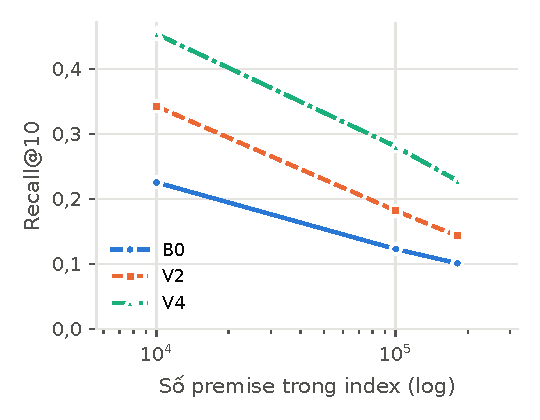
\includegraphics[width=\linewidth]{fig_quality_vs_size.pdf}
  \caption{Recall@10 theo số premise trong chỉ mục}
\end{subfigure}\hfill
\begin{subfigure}[t]{0.49\linewidth}
  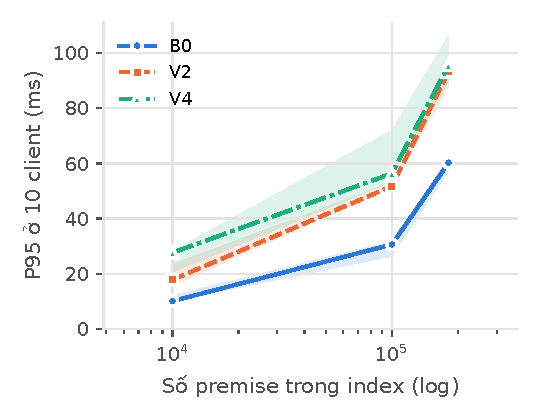
\includegraphics[width=\linewidth]{fig_latency_vs_size.pdf}
  \caption{P95 ở 10 client theo số premise}
\end{subfigure}
\caption[Chất lượng và độ trễ theo kích thước chỉ mục]{Chất lượng và độ trễ theo kích thước chỉ mục (mẫu 500 truy vấn;
vùng tô là khoảng giữa lần nhanh nhất và chậm nhất trong 3 lần).}\label{fig:scale}
\end{figure}

\FloatBarrier
\section{Độ trễ dưới tải đồng thời}\label{sec:load}

Hình~\ref{fig:clients} cho kết quả kiểm tra tải trên chỉ mục đầy đủ với 4 worker. Từ 1 lên 10 client, QPS tăng từ 3 đến
3,5 lần và P95 tăng khoảng 2,5 lần (V4 từ 38,4 lên 95,5 ms). Ở 50 client cả ba hệ thống đều bão hòa: QPS gần như không đổi
và P95 lên 345,9 đến 566,8 ms vì các yêu cầu phải xếp hàng. Trong \num{32400} yêu cầu có 4 yêu cầu lỗi, đều phía client;
khoảng biến thiên tương đối của P95 giữa các lần lặp có trung vị 9\% và lớn nhất 43\%.

\Needspace{5\baselineskip}
\paragraph{Thêm worker có giúp không?} Với 4, 8 và 12 worker và thêm mức 100 client (Bảng~\ref{tab:workers},
Phụ lục~\ref{app:tables}), thông lượng gần như không đổi (B0 khoảng 230 đến 260 QPS, V4 khoảng 140 đến 160 QPS) trong khi
RAM của server tăng từ 3,4 lên 9,8 GB. Ngay với 4 worker, các worker đã dùng 8 đến 9,5 trên 12 luồng logic, và tạo tải bằng
bốn tiến trình client cũng không tăng QPS. Trên máy này dịch vụ bị giới hạn bởi CPU: muốn tăng thông lượng phải giảm chi phí
CPU mỗi truy vấn hoặc thêm máy (chưa đo), còn thêm worker chỉ tốn bộ nhớ.

\Needspace{5\baselineskip}
\paragraph{Đối chiếu với Lucene.} Với BM25 của Lucene 10.5 qua Anserini 2.3.0 trên cùng trường và cùng tập test
(Bảng~\ref{tab:lucene}, Phụ lục~\ref{app:tables}), khi nhận đúng các token của B0 cùng $k_1$ và $b$, Lucene cho các chỉ số rất gần B0 (MRR 0,0657 so
với 0,0654); top 10 trùng trung bình 98,9\% phần tử và trùng nguyên tập ở 89,6\% truy vấn, phần lệch còn lại phù hợp với
việc Lucene nén độ dài tài liệu. Giữ nguyên $k_1$ và $b$, bộ phân tích tiếng Anh làm Recall@10 giảm từ 0,100 xuống 0,089 vì
bỏ stopword và rút gọn từ làm hỏng tên Lean; tham số mặc định của Anserini làm giảm thêm xuống 0,076. Lucene mất 2,4 ms mỗi
truy vấn so với 13,2 ms của B0 đo cùng quy tắc, tức nhanh hơn khoảng 5,5 lần; đây là trung bình khi chạy một thread với cấu hình B0,
chưa phải bằng chứng về BM25F ba trường hay P95 của API sau khi tích hợp Lucene.

\section{Xây chỉ mục theo lô}

Đường xây chỉ mục được đo qua hai đợt. Đợt đầu dùng engine RDD trên chỉ mục B0 với corpus tới \num{904785} bản ghi trên
Windows; bản tuần tự nhanh nhất ở mọi kích thước (ở 905K bản ghi, 17,8 giây so với 41,0 giây của local[4]), vì driver đọc
toàn bộ dữ liệu rồi mới phân phối, mỗi posting là một cặp khóa và giá trị Python phải tuần tự hóa, và job có hai lượt
shuffle lớn. Đợt thứ hai dùng engine Arrow cho chỉ mục B0 và chỉ mục ba trường, với corpus tới 3,6 triệu bản ghi, trên
Windows và trong container Linux trên cùng phần cứng; cả 194 lần chạy đều thành công và mọi cách xây cho cùng mã SHA-1 của
từng tệp chỉ mục.

\input{tables/build}

\begin{figure}[htbp]
\centering
\begin{subfigure}[t]{0.49\linewidth}
  \includegraphics[width=\linewidth]{fig_build2_time_lean.pdf}
  \caption{Thời gian xây chỉ mục ba trường}
\end{subfigure}\hfill
\begin{subfigure}[t]{0.49\linewidth}
  \includegraphics[width=\linewidth]{fig_build2_speedup.pdf}
  \caption{Tăng tốc so với bản tuần tự, chỉ mục ba trường}
\end{subfigure}
\caption[Xây chỉ mục bằng engine Arrow]{Xây chỉ mục bằng engine Arrow theo kích thước corpus (trục hoành logarit; hai mức
cuối là corpus nhân bản 5 và 20 lần, chỉ dùng để đo thời gian, bộ nhớ và độ lệch).}\label{fig:build}
\end{figure}

\paragraph{Điểm giao nhau.} Ở kích thước nhỏ, chi phí cố định của Spark (khởi động phiên khoảng 4 giây, tạo tiến trình
Python cho mỗi task) chiếm phần lớn thời gian, nhất là trên Windows, nơi PySpark không fork được worker. Khi corpus lớn lên,
phần tính toán lấn át chi phí cố định (Bảng~\ref{tab:build}, Hình~\ref{fig:build}). Trên corpus mathlib4 thật (181K premise),
Spark local[8] chỉ nhanh hơn bản tuần tự với chỉ mục ba trường trên Linux (1,53 lần); trên corpus nhân bản 3,6 triệu bản
ghi, nhanh hơn 3,84 lần trên Linux và 2,96 lần trên Windows. Các mức này đo bằng Spark chế độ local trên một máy 6 nhân,
nên chứng minh lợi ích của song song hóa cục bộ chứ chưa phải khả năng mở rộng trên cụm, và corpus nhân bản giữ nguyên số
khóa nên thuận lợi cho engine Arrow.

\paragraph{Số thread, bộ nhớ và độ ổn định.} Ở 3,6 triệu bản ghi trên Linux, thời gian giảm từ 238,5 giây (local[2]) xuống
95,6 giây (local[8]) còn RAM đỉnh tăng từ mức của bản tuần tự (5,0 GB) lên 8,2 GB. Ở 58 trên 64 cấu hình, các lần lặp chênh
nhau không quá 5\% trung vị. Hai nền tảng chạy Python khác phiên bản nên chỉ so sánh trong cùng một nền tảng.

% ================================================================ 7
\chapter{Ablation, phân tích lỗi và hạn chế}\label{sec:ablation}

\section{Ablation của reranker}\label{sec:ablation-rerank}

Mỗi biến thể trong Bảng~\ref{tab:ablation} bỏ đúng một nhóm đặc trưng hoặc đổi đúng một tham số của V4, rồi huấn luyện
lại reranker trên cùng dữ liệu. Giả thuyết và quy tắc kết luận được ghi trong \code{docs/ablation\_plan.md}: thành phần có
tác dụng nếu $p$ sau hiệu chỉnh Holm nhỏ hơn 0,05; ngược lại kết luận là không phân biệt được, không phải là vô dụng.

\input{tables/ablation}

\input{tables/controls}

Bộ lọc accessible premise là thành phần có giá trị nhất; tiếp theo là điểm của giai đoạn 1 và cặp đặc trưng phụ thuộc. Sau
hiệu chỉnh Holm, bỏ độ trùng ký hiệu ($-0{,}009$) và giảm xuống 50 candidate ($-0{,}009$) không còn có ý nghĩa với
Recall@10 ($p$ Holm bằng 0,132), dù vẫn có ý nghĩa với MRR. Đặc trưng vị trí và loại khai báo không làm thay đổi Recall@10
nhưng làm giảm MRR có ý nghĩa khi bị bỏ, nghĩa là chúng giúp đưa gold premise lên đầu danh sách mà không đưa thêm gold
premise vào top 10. Đặc trưng namespace của reranker không có tác dụng đo được ở cả hai chỉ số. Tăng số candidate lên 200 làm
Recall@10 tăng 0,010 ($p$ Holm bằng 0,019); V4 giữ 100 candidate vì giá trị này đã được chốt trước khi chạy tập test.

\Needspace{5\baselineskip}
Bảng~\ref{tab:controls} tách thêm hai thành phần mà ablation trên chưa tách. Bỏ trường namespace khỏi BM25F, một can thiệp
khác với bỏ đặc trưng namespace của reranker, không tạo khác biệt có ý nghĩa trên \code{random}. Giữ riêng popularity hoặc
riêng PageRank cho Recall@10 trong khoảng 0,002 quanh V4 với khoảng tin cậy chứa 0.

\FloatBarrier

\section{Ablation của đường xây chỉ mục}

\paragraph{Hai engine Spark.}\label{sec:engines} Trên cùng chỉ mục B0 với Spark local[4] (Bảng~\ref{tab:engines}, Phụ
lục~\ref{app:tables}), engine Arrow nhanh hơn engine RDD 1,7 lần ở 905K và 3,0 lần ở 3,6 triệu bản ghi, và cần ít RAM hơn
3 đến 6 lần vì driver của engine RDD phải giữ toàn bộ dữ liệu đầu vào. Dung lượng shuffle sau nén của hai engine tương
đương (183 MB và 204 MB ở 3,6 triệu bản ghi); khác biệt nằm ở số bản ghi Python phải tuần tự hóa: khoảng 67 triệu cặp
khóa và giá trị ở engine RDD so với khoảng 0,5 triệu bản ghi ở engine Arrow.

\paragraph{Kết hợp cục bộ và tách khóa nóng.} Với engine RDD ở 905K bản ghi, bỏ kết hợp cục bộ làm dữ liệu shuffle tăng
2,5 lần (từ 52,1 lên 130,7 MB) và thời gian tăng từ 41,0 lên 58,3 giây. Tách khóa nóng thành 4 phần giảm thời gian của task
reduce chậm nhất từ 6,4 xuống 4,2 giây nhưng cần thêm hai pha, nên tổng thời gian tăng lên 53,5 giây. Ở quy mô này độ lệch
chưa đủ lớn để việc tách khóa có lợi.

\paragraph{Cách mã posting list.} Với chỉ mục B0 khi tắt bộ đệm, dung lượng posting là 12,8 MB với số nguyên 32 bit,
4,1 MB với VB và 2,6 MB với gamma; P50 truy vấn tương ứng là 12,7; 16,9 và 137,7 ms. VB nhỏ hơn 3,1 lần so với số nguyên 32
bit và chỉ chậm hơn 4 ms, còn gamma chậm hơn VB khoảng 8 lần vì giải mã từng bit bằng Python. Khi bật bộ đệm như cấu hình
mặc định, cả ba có trung vị độ trễ từ 12,9 đến 13,4 ms và cho cùng kết quả truy hồi.

\section{Phân tích lỗi}\label{sec:errors}

Trên tập test \code{random}, V4 không đưa được \num{4369} trong \num{5483} cặp (truy vấn, gold premise) vào top 10.
Bảng~\ref{tab:errors} phân loại tự động các cặp này; một cặp có thể thuộc nhiều nhóm. Phân tích này được làm trên tập test và đã dẫn tới thiết kế của V5 (Mục~\ref{sec:holdout}).

\input{tables/errors}

Phát hiện quan trọng nhất là 82,7\% cặp bị bỏ lỡ nằm ngoài 100 candidate của giai đoạn 1, nên reranker không thể cứu
được. Các premise tổng quát như bổ đề về $\le$, $+$ hay $\in$ được dùng ở rất nhiều nơi nhưng ít trùng từ với một proof
state cụ thể, và gần một phần tư premise bị bỏ lỡ không có từ nào chung với truy vấn. Đây là những trường hợp dense
retrieval có khả năng bổ sung tốt. Theo lát cắt, V4 tốt hơn B0 ở mọi lĩnh vực có ít nhất 30 truy vấn; mức tăng Recall@10 lớn nhất
ở LinearAlgebra (0,201) và FieldTheory (0,163), nhỏ nhất ở Combinatorics (0,049) và NumberTheory (0,059). Truy vấn ngắn từ
20 token trở xuống dễ nhất với Recall@10 bằng 0,378, truy vấn dài hơn 160 token khó nhất với 0,169, và truy vấn cần từ 5
premise trở lên chỉ đạt 0,120.

Bảng~\ref{tab:example} theo dõi ví dụ xuyên suốt qua từng biến thể. Gold premise \code{mul\_assoc} không có từ nào chung
với proof state ngoài các ký hiệu \code{*} và \code{=}, nên B0 đến V4 đều không đưa nó vào 100 candidate; các biến thể này
trả về những bổ đề về \code{invOf} có tên gần với proof state. V5 đưa nó vào candidate pool qua nguồn theo tệp, vì một
theorem train A khai báo trước trong cùng tệp đã dùng nó, và reranker xếp nó ở hạng 2; \code{mul\_assoc} cũng là premise
được dùng nhiều thứ tư trong train A. Ví dụ này minh họa cơ chế, không phải bằng chứng định lượng; Mục~\ref{sec:robust}
cho thấy cùng cơ chế đó làm giảm recall trên unseen premise.

\input{tables/example}

\paragraph{Tạo candidate hay xếp hạng.} Bảng~\ref{tab:candidates} tách phần recall bị mất thành candidate loss và
ranking gap. Với V4, candidate loss (0,603 trên \code{random}) lớn gấp khoảng bốn lần ranking gap (0,154), đúng như phân
tích lỗi ở trên. Với V5, candidate recall tăng lên 0,650 nhưng ranking gap tăng lên 0,369, xấp xỉ candidate loss (0,350):
phần lớn gold premise mới vào candidate pool vẫn bị reranker tuyến tính xếp ngoài top 10. Trong các gold premise nằm trong candidate pool
của V5 trên \code{random}, 55,6\% đến từ BM25F, 23,1\% từ nguồn theo tệp, 10,9\% từ nguồn theo thư mục và 10,3\% từ nguồn phổ
biến. Như vậy reranker trở thành một hướng cải thiện quan trọng ngang với bước tạo candidate, nhưng bước tạo candidate vẫn bỏ
lỡ khoảng 35\% gold premise.

\input{tables/candidates}

\Needspace{6\baselineskip}
\paragraph{Gán nhãn thủ công.} Ngoài phân loại tự động, nhóm đã lấy mẫu phân tầng 30 trường hợp thất bại kèm proof state,
gold premise, hạng của nó và ba kết quả đầu của V4 (\code{results/figures/failure\_cases.md}). Kế hoạch là hai thành viên
gán nhãn độc lập theo cùng bảng nhóm lỗi, rồi đối chiếu và báo tỉ lệ đồng thuận thô; việc gán nhãn này chưa được thực
hiện.

\section{Một lỗi được phát hiện nhờ phân tích lỗi}\label{sec:bug}

Phiên bản đầu của bộ lọc accessible premise so dòng \emph{bắt đầu} của premise cùng tệp với dòng bắt đầu của theorem. Vì
vị trí của một khai báo trong dữ liệu tính cả docstring và thuộc tính đứng trước nó, chính theorem đang chứng minh có thể
có dòng bắt đầu nhỏ hơn dòng bắt đầu được ghi cho truy vấn và lọt qua bộ lọc. Lỗi này xảy ra ở \num{1111} trên
\num{2641} truy vấn của tập test, tức 42\%. Nhóm phát hiện lỗi khi thấy chính theorem đang chứng minh xuất hiện trong
danh sách candidate. Bộ lọc được sửa để so dòng kết thúc, có thêm test hồi quy kiểm tra rằng theorem không bao giờ là
accessible premise của chính nó và mọi gold premise của tập test đều là accessible premise. V2a và V4 đã được huấn luyện và đánh giá lại;
mọi số liệu trong báo cáo là sau khi sửa.

\section{Hạn chế và threats to validity}

\paragraph{Phạm vi của benchmark.} Benchmark chỉ tính premise có trong corpus, nên recall báo cáo cao hơn recall mà bộ
chứng minh gặp thực tế; kết quả cũng chỉ đại diện cho 44,1\% theorem trong tập test \code{random} còn truy vấn sau lọc. So
sánh giữa các biến thể vẫn công bằng vì dùng cùng định nghĩa và cùng tập truy vấn.

\paragraph{Tập test tham gia thiết kế.} V5 được thiết kế từ phân tích lỗi trên tập test \code{random}, nên kết quả của V5
trên tập test có được sau khi đã xem lỗi trên chính tập đó. Holdout lấy từ phần train B chưa dùng để huấn luyện reranker,
cùng snapshot và có ít truy vấn mỗi theorem hơn tập test, nên không chứng minh khả năng tổng quát hóa sang phiên bản thư
viện khác. Tham số của giai đoạn 1 được chọn trên một lưới giới hạn; với V2, cấu hình được chọn thấp hơn điểm tốt nhất trên
validation 0,0005 theo một quy tắc không định trước.

\paragraph{Tương quan và nhiều phép so sánh.} Các truy vấn của cùng một theorem không độc lập: bootstrap theo cụm cho khoảng
tin cậy rộng hơn bootstrap theo truy vấn, và theorem-macro đổi dấu chênh lệch giữa V4 và V5 trên \code{novel\_premises}.
Kiểm định hoán vị giả định các theorem hoán đổi được độc lập. Nhóm phép so sánh chính và ablation đã hiệu chỉnh Holm; các
so sánh phụ thì chưa, nên một kết quả phụ có $p$ gần 0,05 chỉ là gợi ý. Ablation của V4, V4-poponly và V4-pronly chỉ chạy
trên \code{random}; V2-nons có cả hai split, còn V4-K240 có cả hai split và holdout.

\paragraph{Prior tĩnh.} Popularity và PageRank tính một lần trên train A, không theo vị trí của từng truy vấn. Điều này hợp
lệ với benchmark tĩnh nhưng không mô phỏng việc viết một định lý mới tại một thời điểm.

\paragraph{Một máy, chế độ local, corpus nhân bản.} Mọi phép đo thời gian thực hiện trên một máy 6 nhân, kể cả thí nghiệm
Linux trong container, nên chưa phản ánh chi phí mạng và điều phối của một cụm; chương trình tạo tải cũng chạy cùng máy với
server. Corpus gấp 5 và gấp 20 lần giữ nguyên phân phối term và số khóa, nên posting list dài và đều hơn dữ liệu thật; trên
một corpus thật lớn cỡ đó, mức giảm bản ghi shuffle của engine Arrow sẽ nhỏ hơn.

\paragraph{Truy vết phiên bản mã.} Các bản ghi lần chạy ghi phiên bản mã là \code{uncommitted} kèm mã băm của mã nguồn, vì
kho mã chưa được commit tại thời điểm chạy. Bảng và hình của báo cáo đọc các lần chạy đã ghim trong
\path{results/figures/report_manifest.json} và \path{report_records.json}; khi commit, các lần chạy cũ sẽ không được sửa hồi
tố mà các lần chạy lại sẽ ghi mã commit đầy đủ.

% ================================================================ 8
\chapter{Kết luận và hướng phát triển}\label{sec:conclusion}

Với RQ1, BM25 mặc định chưa đủ cho dữ liệu Lean. Việc tinh chỉnh tham số, sử dụng trường name và đặc biệt là thông tin
phụ thuộc có tác dụng đo được; với tokenizer Lean (trên Recall@10) và trường namespace thì chưa có đủ bằng chứng, còn popularity và PageRank chỉ
kết luận được theo cặp. Với RQ2, kết hợp BM25F với các đặc trưng cấu trúc (V4) đưa Recall@10 từ 0,100 lên 0,243 trên tập
test \code{random} và từ 0,127 lên 0,269 trên \code{novel\_premises}; trong đợt đo tải chính, P95 latency ở 10 client tăng từ
60,2 lên 95,5 ms, phần lớn do giai đoạn BM25F, còn các đặc trưng cấu trúc chỉ tốn khoảng 2 ms. V4 là lựa chọn cân bằng giữa
chất lượng và độ trễ. V5 bổ sung candidate từ lịch sử sử dụng, nâng Recall@10 trên \code{random} lên 0,281 và hơn V4 trên
holdout (0,332 so với 0,310); tuy nhiên trên holdout chưa có đủ bằng chứng cho thấy V5 tốt hơn V4-K240, V5 làm giảm recall
trên unseen premise của \code{novel\_premises}, và có chi phí rõ hơn khi tải cao. V5 vì vậy là một đánh đổi có lợi cho
premise quen thuộc. Về phục vụ, dịch vụ bị giới hạn bởi CPU của máy; BM25 của Lucene cho kết quả rất gần B0 và nhanh hơn
khoảng 5,5 lần khi chạy một thread. Về khía cạnh dữ liệu lớn, chỉ mục xây
bằng Spark trùng từng byte với bản tuần tự. Engine RDD ban đầu không nhanh hơn bản tuần tự ở kích thước nào; sau khi viết
lại với lô Arrow và gộp posting theo partition, Spark local[8] nhanh hơn bản tuần tự 1,53 lần trên corpus thật 181K (Linux,
chỉ mục ba trường) và 3,84 lần trên corpus nhân bản 3,6 triệu bản ghi, đều trên một máy. Cách tổ chức job, đặc biệt là gộp
dữ liệu trước khi shuffle, quyết định lợi ích của xử lý song song.

Sản phẩm bàn giao gồm đặc tả benchmark, gói benchmark chung với Nhóm 4, pipeline trích xuất có kiểm tra chất lượng, chỉ mục đảo tái tạo được kèm manifest,
dịch vụ truy vấn qua API và CLI, baseline BM25, reranker cấu trúc, các script đánh giá, ablation và phân tích lỗi, README
và kịch bản demo. Các bảng và hình của báo cáo được sinh bằng script từ kết quả thô và các lần chạy đã ghim; nguồn của
từng bảng, từng hình và mã SHA-256 của đầu vào ghi trong \code{tables/SOURCES.md} và \code{figures/SOURCES.md}. Các việc còn phải do thành viên thực
hiện gồm đối chiếu thủ công 20 truy vấn kiểm tra, gán nhãn 30 trường hợp thất bại và so sánh với Nhóm 4.

Nhóm đề xuất năm hướng tiếp theo. Thứ nhất, trộn kết quả với hệ thống dense retrieval của Nhóm 4 bằng Reciprocal Rank Fusion
thành hybrid retrieval, để tìm các premise không có từ chung với truy vấn và các unseen premise. Thứ hai, thay reranker tuyến tính bằng một mô hình xếp
hạng phi tuyến, chọn trên validation và kiểm tra trên một holdout mới, vì Oracle@10 của V5 là 0,650 trong khi Recall@10 mới
đạt 0,281; mô hình này cần giữ được recall trên unseen premise. Thứ ba, thay giai đoạn 1 bằng Lucene hoặc cài đặt các
kỹ thuật dừng sớm như MaxScore và WAND~\cite{broder2003}, rồi đo lại P95 của API. Thứ tư, chạy thí nghiệm xây chỉ mục trên
cụm nhiều máy với corpus thật lớn hơn. Thứ năm, tích hợp với một bộ chứng minh Lean để đo ảnh hưởng của chất lượng truy hồi
tới tỉ lệ chứng minh thành công.

% ================================================================ Tài liệu tham khảo
\begingroup\small
\setlength{\itemsep}{1pt}
\begin{thebibliography}{99}
\setlength{\itemsep}{1pt}
\phantomsection\addcontentsline{toc}{chapter}{Tài liệu tham khảo}
\bibitem{demoura2021} L. de Moura, S. Ullrich. The Lean 4 Theorem Prover and Programming Language. \emph{Automated
Deduction, CADE 28}, Lecture Notes in Computer Science 12699, Springer, 2021.
\bibitem{mathlib2020} The mathlib Community. The Lean Mathematical Library. \emph{Proceedings of the 9th ACM SIGPLAN
International Conference on Certified Programs and Proofs (CPP)}, 2020.
\bibitem{yang2023} K. Yang, A. Swope, A. Gu, R. Chalamala, P. Song, S. Yu, S. Godil, R. Prenger, A. Anandkumar.
LeanDojo: Theorem Proving with Retrieval-Augmented Language Models. \emph{Advances in Neural Information Processing
Systems 36 (NeurIPS), Datasets and Benchmarks Track}, 2023.
\bibitem{leandojodocs} LeanDojo documentation. \url{https://leandojo.readthedocs.io/}. Truy cập tháng 10/2026.
\bibitem{robertson2009} S. Robertson, H. Zaragoza. The Probabilistic Relevance Framework: BM25 and Beyond.
\emph{Foundations and Trends in Information Retrieval} 3(4), 2009.
\bibitem{manning2008} C. D. Manning, P. Raghavan, H. Schütze. \emph{Introduction to Information Retrieval}. Cambridge
University Press, 2008.
\bibitem{scholer2002} F. Scholer, H. E. Williams, J. Yiannis, J. Zobel. Compression of Inverted Indexes for Fast Query
Evaluation. \emph{Proceedings of the 25th ACM SIGIR Conference}, 2002.
\bibitem{meng2009} J. Meng, L. C. Paulson. Lightweight Relevance Filtering for Machine-Generated Resolution Problems.
\emph{Journal of Applied Logic} 7(1), 2009.
\bibitem{irving2016} G. Irving, C. Szegedy, A. A. Alemi, N. Eén, F. Chollet, J. Urban. DeepMath: Deep Sequence Models for
Premise Selection. \emph{Advances in Neural Information Processing Systems 29 (NeurIPS)}, 2016.
\bibitem{mikula2024} M. Mikuła và cộng sự. Magnushammer: A Transformer-Based Approach to Premise Selection.
\emph{International Conference on Learning Representations (ICLR)}, 2024. arXiv:2303.04488.
\bibitem{dean2004} J. Dean, S. Ghemawat. MapReduce: Simplified Data Processing on Large Clusters. \emph{6th Symposium on
Operating Systems Design and Implementation (OSDI)}, 2004.
\bibitem{zaharia2012} M. Zaharia và cộng sự. Resilient Distributed Datasets: A Fault-Tolerant Abstraction for In-Memory
Cluster Computing. \emph{9th USENIX Symposium on Networked Systems Design and Implementation (NSDI)}, 2012.
\bibitem{sparkdocs} Apache Spark documentation. \url{https://spark.apache.org/docs/latest/}. Truy cập tháng 10/2026.
\bibitem{lin2010} J. Lin, C. Dyer. \emph{Data-Intensive Text Processing with MapReduce}. Morgan \& Claypool, 2010.
\bibitem{page1999} L. Page, S. Brin, R. Motwani, T. Winograd. The PageRank Citation Ranking: Bringing Order to the Web.
Technical Report, Stanford InfoLab, 1999.
\bibitem{cormack2009} G. V. Cormack, C. L. A. Clarke, S. Büttcher. Reciprocal Rank Fusion Outperforms Condorcet and
Individual Rank Learning Methods. \emph{Proceedings of the 32nd ACM SIGIR Conference}, 2009.
\bibitem{zenodo2024} K. Yang. LeanDojo Benchmark 4, phiên bản v10. Zenodo, 2024. \url{https://zenodo.org/records/12740403}.
\bibitem{mathlib4repo} mathlib4. \url{https://github.com/leanprover-community/mathlib4}. Truy cập tháng 10/2026.
\bibitem{efron1993} B. Efron, R. J. Tibshirani. \emph{An Introduction to the Bootstrap}. Chapman \& Hall, 1993.
\bibitem{good2005} P. Good. \emph{Permutation, Parametric, and Bootstrap Tests of Hypotheses}, ấn bản 3. Springer, 2005.
\bibitem{phipson2010} B. Phipson, G. K. Smyth. Permutation P-values Should Never Be Zero: Calculating Exact P-values When
Permutations Are Randomly Drawn. \emph{Statistical Applications in Genetics and Molecular Biology} 9(1), 2010.
\bibitem{holm1979} S. Holm. A Simple Sequentially Rejective Multiple Test Procedure. \emph{Scandinavian Journal of
Statistics} 6(2), 1979.
\bibitem{broder2003} A. Z. Broder, D. Carmel, M. Herscovici, A. Soffer, J. Zien. Efficient Query Evaluation Using a
Two-Level Retrieval Process. \emph{Proceedings of the 12th ACM CIKM}, 2003.
\end{thebibliography}
\endgroup

% ================================================================ Phụ lục
\appendix
\chapter{Khai báo sử dụng AI và đóng góp}\label{app:aicontrib}

\section{Khai báo sử dụng AI}\label{app:ai}

Theo yêu cầu học phần, nhóm khai báo việc sử dụng công cụ AI như sau.

\begin{center}
\renewcommand{\arraystretch}{1.3}
\begin{tabularx}{\linewidth}{|>{\raggedright\arraybackslash}p{2.15cm}|>{\raggedright\arraybackslash}p{3.1cm}|>{\raggedright\arraybackslash}p{4.4cm}|>{\raggedright\arraybackslash}X|}
\hline
\rowcolor{black!12}\textbf{Hạng mục} & \textbf{Công cụ} & \textbf{Phần được hỗ trợ} & \textbf{Cách nhóm kiểm chứng} \\
\hline
Mã nguồn & Claude (Anthropic) qua Claude Code & Khung mã các module trích xuất, xây chỉ mục, BM25/BM25F, reranker,
dịch vụ và đánh giá; script thí nghiệm & Chạy toàn bộ 68 unit test; so SHA-1 chỉ mục Spark $\leftrightarrow$ tuần tự trùng
từng byte; đối chiếu BM25 với Lucene; test hồi quy bộ lọc accessible premise \\
\hline
\end{tabularx}
\end{center}

\section{Phân công và đóng góp}\label{app:contrib}

Mỗi vai trò có một người chính và một người dự phòng có thể chạy lại và giải thích phần việc khi bảo vệ
(Bảng~\ref{tab:roles}). Nhật ký đóng góp chi tiết nằm trong tệp \code{contributions.md}.

\begin{table}[H]
\centering
\caption{Vai trò, người phụ trách và phần mã tương ứng}\label{tab:roles}
\small
\begin{tabularx}{\linewidth}{@{}>{\raggedright\arraybackslash}p{2.5cm}>{\raggedright\arraybackslash}p{2.8cm}l>{\raggedright\arraybackslash}p{2.8cm}>{\raggedright\arraybackslash}X@{}}
\toprule
Vai trò & Người chính & Mã SV & Dự phòng & Phần phụ trách \\
\midrule
Dữ liệu và trích xuất & Nguyễn Đức Hoàng & B25CHHT096 & Nguyễn Ngọc Minh & tải dữ liệu, trích xuất, tập con, data card, data dictionary, 20 truy vấn kiểm tra \\
Xây chỉ mục & Trần Duy Khánh & B25CHHT100 & Vũ Trung Kiên & xây chỉ mục tuần tự và Spark, nén posting, thí nghiệm xây chỉ mục \\
Baseline BM25 & Nguyễn Mạnh Cường & B25CHHT082 & Trần Đình Dũng & tokenizer, BM25 và BM25F, tinh chỉnh tham số, đối chiếu Lucene \\
Đặc trưng cấu trúc & Trần Đình Dũng & B25CHHT089 & Nguyễn Mạnh Cường & đặc trưng, bộ lọc accessible premise, thống kê phụ thuộc, reranker, V5 \\
Phục vụ và hiệu năng & Vũ Trung Kiên & B25CHHT101 & Trần Duy Khánh & API, CLI, kiểm tra tải, profile độ trễ \\
Đánh giá và phân tích lỗi & Nguyễn Ngọc Minh & B25CHHT106 & Nguyễn Đức Hoàng & chỉ số, kiểm định, ablation, phân tích lỗi, holdout, so sánh với Nhóm 4, báo cáo \\
\bottomrule
\end{tabularx}
\end{table}

\chapter{Tái lập kết quả}\label{app:reproduce}

\section{Lệnh tái lập}\label{app:repro}

Các lệnh dưới đây chạy trong thư mục gốc của kho mã, với môi trường cài theo \code{README.md}. Để dựng lại đúng bản đã
phát hành, chạy \code{build.sh}: lệnh này không chạy lại thí nghiệm, chỉ đọc các lần chạy đã ghim, và trước khi sinh lại bảng
và hình sẽ so SHA-256 của mọi tệp đầu vào với \path{tables/SOURCES.md}, \path{figures/SOURCES.md}, dừng nếu có tệp lệch. Để
tái tạo từ đầu, chạy \code{scripts/reproduce.sh}; script này ghim lại các lần chạy mới nhất rồi dựng báo cáo bằng
\code{build.sh -{}-update}, nên bảng có thể thay đổi. Các tùy chọn \code{-{}-with-tuning}, \code{-{}-with-scale} chạy lại quá
trình chọn tham số và các thí nghiệm quy mô, tải, Lucene.

\begin{Verbatim}[fontsize=\footnotesize,frame=single,framesep=2mm,commandchars=\\\{\}]
\textrm{\# dựng lại đúng bản đã phát hành từ các lần chạy đã ghim}
python -m pytest -q                                   \textrm{\# 68 unit test}
bash report/latex/build.sh                 \textrm{\# hoặc --compile-only: chỉ biên dịch}

\textrm{\# tái tạo từ đầu, ghim lại lần chạy mới nhất rồi dựng báo cáo}
bash scripts/reproduce.sh [--with-tuning] [--with-scale] [--report]

\textrm{\# một biến thể trên một tập, và truy vấn thử}
python -m eval.run_eval --config configs/v4_rerank_dep.yaml \textbackslash
    --eval random_test_all
python -m serving.cli --query-id random:val:36:0 --mode V5 -k 5
uvicorn serving.api:app --port 8000 --workers 4
python scripts/eval_shared.py [--external N4-dense=<run>.csv]  \textrm{\# benchmark chung với Nhóm 4}

\textrm{\# cập nhật phân tích sau khi có lần chạy mới (thay đổi bản đã ghim)}
python scripts/pin_runs.py && python scripts/ablation_significance.py
python scripts/robustness.py && python scripts/candidate_analysis.py
bash report/latex/build.sh --update

\textrm{\# xây chỉ mục trên Linux, cùng máy}
docker build -t n3-spark-linux -f docker/spark-linux.Dockerfile docker
docker run --rm -v <repo>:/repo n3-spark-linux \textbackslash
    bash /repo/docker/run_build2_linux.sh --reps 3 --sizes 10k,full,x5,x20
\end{Verbatim}

Bảng nào được sinh từ tệp kết quả nào, các \code{run\_id} đã ghim và mã SHA-256 của mọi tệp đầu vào tại thời điểm sinh
bảng được liệt kê trong \code{report/latex/tables/SOURCES.md}; thứ tự thời gian của các lần chạy nằm trong
\code{docs/process\_log.md}.

\Needspace{14\baselineskip}
\section{Ví dụ một bản ghi lần chạy}\label{app:record}

Bản ghi dưới đây của lần đánh giá V5 trên tập holdout được rút gọn; bản đầy đủ gồm cả cấu hình, thông tin chỉ mục và mọi
chỉ số nằm trong \code{results/raw/eval}.

\noindent\begin{minipage}{\linewidth}
\begin{Verbatim}[fontsize=\footnotesize,frame=single,framesep=2mm]
{"run_id": "eval-V5-20261018-230340-4bf3", "kind": "eval",
 "timestamp": "2026-10-18T16:04:39+00:00", "git_commit": "uncommitted",
 "code_hash": "50e9470e64ad", "data_version": "leandojo_benchmark_4@v10#md5:25e1ee60",
 "parameters": {"config": {"name": "V5"}, "eval_set": "random_holdoutB"},
 "seed": 42, "status": "ok",
 "metrics": {"R@10": 0.3323, "MRR": 0.2609, "n_queries": 2500}}
\end{Verbatim}
\end{minipage}

\chapter{Bảng bổ sung}\label{app:tables}

Các bảng dưới đây bổ sung cho phần thân và được nhắc tới trong các chương tương ứng, xếp theo ba nhóm.

\section{Dữ liệu và môi trường}

\begin{table}[htbp]
\centering
\caption{Nguồn dữ liệu}\label{tab:source}
\begin{tabularx}{\linewidth}{@{}lX@{}}
\toprule
Thuộc tính & Giá trị \\
\midrule
Bộ dữ liệu & LeanDojo Benchmark 4, phiên bản v10, công bố ngày 14/7/2024 \\
Nơi tải & Zenodo record 12740403, tệp \code{leandojo\_benchmark\_4.tar.gz}, md5 \code{25e1ee60cd8925b9d2e8673ddcc34b4c} \\
Phiên bản thư viện & mathlib4 commit \code{29dcec07}, trích bằng LeanDojo 2.0.0~\cite{mathlib4repo} \\
Giấy phép & Bộ dữ liệu: CC BY 2.0. Mã nguồn Lean của mathlib4, Lean 4 và Batteries: Apache 2.0 \\
Nội dung & \code{corpus.jsonl} (khai báo theo tệp), các tệp \code{train/val/test.json} của hai split \\
\bottomrule
\end{tabularx}
\end{table}

\begin{table}[htbp]
\centering
\caption[Các bảng sau trích xuất]{Các bảng sau trích xuất. Bảng \code{queries} chứa truy vấn của cả hai split, nên
một tactic thuộc cả hai split được đếm hai lần}\label{tab:schema}
\begin{tabularx}{\linewidth}{@{}lr>{\raggedright\arraybackslash}p{2.6cm}X@{}}
\toprule
Bảng & Số dòng & Khóa & Cột chính \\
\midrule
\code{premises} & \num{180957} & \code{premise\_id} & tên đầy đủ, tệp, namespace, loại khai báo, phát biểu, mã nguồn, dòng bắt đầu và kết thúc \\
\code{queries} & \num{315014} & \code{query\_id} & split, theorem đang chứng minh, tệp, dòng bắt đầu, proof state \\
\code{qrels} & \num{674628} & (\code{query\_id}, \code{premise\_id}) & nhãn liên quan nhị phân \\
\code{files} & \num{5674} & \code{path} & danh sách tệp được import trực tiếp \\
\code{dead\_letter} & \num{136296} & \code{key} & loại bản ghi bị loại và lý do \\
\bottomrule
\end{tabularx}
\end{table}

\begin{table}[htbp]
\centering
\caption{Môi trường thí nghiệm}\label{tab:env}
\begin{tabularx}{\linewidth}{@{}lX@{}}
\toprule
Thành phần & Cấu hình \\
\midrule
CPU & Intel Core thế hệ 12 (Alder Lake), 6 nhân vật lý, 12 luồng \\
Bộ nhớ, hệ điều hành & 32 GB RAM; Windows 11 (bản 26300) \\
Python chính & Python 3.13.0; numpy 2.5.4; pyarrow 26.0.0; pandas 3.0.6; scikit-learn 1.9.1; FastAPI 0.143.3; uvicorn 0.54.0 \\
Spark & PySpark 4.0.1 chạy chế độ local với Python 3.11.17 và Java 21.0.6 (PySpark trên Windows không chạy được với Python 3.13) \\
Linux & container Docker trên cùng máy (máy ảo WSL2 được cấp 12 luồng và 16 GB RAM), Debian 12, Python 3.11.17, Java 17, cùng phiên bản PySpark, numpy, pyarrow và pandas (\code{docker/spark-linux.Dockerfile}) \\
Lucene & Anserini 2.3.0 (Lucene 10.5) trên Java 21.0.6 \\
Lặp và seed & seed 42 cho mọi lấy mẫu; thí nghiệm thời gian lặp 3 lần, báo trung vị cùng giá trị nhỏ nhất và lớn nhất \\
Giới hạn thời gian & mỗi yêu cầu của client kiểm tra tải có timeout 120 giây \\
\bottomrule
\end{tabularx}
\end{table}

\FloatBarrier
\section{Truy hồi, phục vụ và xây chỉ mục}

\input{tables/leandojo}

\input{tables/shared}

\input{tables/v5grid}

\input{tables/lucene}

\input{tables/profile}

\input{tables/workers}

\input{tables/engines}

\clearpage
\section{Thiết kế thí nghiệm}

\begin{table}[htbp]
\centering
\caption[Thiết kế thí nghiệm]{Thiết kế thí nghiệm và số lần chạy, đếm từ các bản ghi trong \code{results/raw}; các lần
chạy ở mức 50K không đưa vào báo cáo. Một lần đo
tải là một mức client của một cấu hình trong một lần lặp, gồm 400 yêu cầu được tính}\label{tab:design}
\begin{tabularx}{\linewidth}{@{}lXr@{}}
\toprule
Thí nghiệm & Các mức & Số lần chạy \\
\midrule
Chất lượng & 8 biến thể; validation và kiểm tra của \code{random}, kiểm tra của \code{novel\_premises} & 24 \\
Đối chứng và holdout & V4-K240 trên 4 tập, V2-nons trên 3 tập, V4-poponly và V4-pronly trên validation và kiểm tra \code{random}; B0, V2, V4, V5 trên holdout & 15 \\
Chất lượng theo quy mô & B0, V2, V4; chỉ mục 10K, 100K, 181K; mẫu 500 truy vấn & 9 \\
Xây chỉ mục, engine RDD & chỉ mục B0; tuần tự, Spark local[2], local[4], local[8]; 10K, 100K, 181K, 905K; Windows; 3 lần & 48 \\
Ablation engine RDD & không kết hợp cục bộ và tách khóa nóng 4 phần (181K, 905K, local[4]); codec raw32 và gamma (181K, tuần tự); 3 lần & 18 \\
Xây chỉ mục, engine Arrow & chỉ mục B0 và ba trường; tuần tự, Spark local[2], local[4], local[8]; 10K, 181K, 905K, 3,6 triệu; Windows và Linux; 3 lần & 192 \\
Engine RDD ở 3,6 triệu & chỉ mục B0, Spark local[4]; Windows và Linux & 2 \\
Tải & B0, V2, V4; 3 kích thước chỉ mục; 1, 10, 50 client; 3 lần (27 cấu hình, \num{32400} yêu cầu) & 81 lần đo \\
Tải theo số worker & B0, V2, V4; 4, 8, 12 worker; 1, 10, 50, 100 client; chỉ mục đầy đủ; 3 lần & 108 lần đo \\
Kiểm tra CPU khi chịu tải & B0; 4, 8, 12 worker; một và bốn tiến trình client & 6 lần đo \\
Tải V4, V4-K240, V5 & cùng server 4 worker; 1, 10, 50 client; 3 lần, thứ tự xoay vòng (thêm 18 lần đo V4, V5 ở phiên trước) & 27 lần đo \\
Ablation reranker & V4 đầy đủ và 9 biến thể, mỗi biến thể huấn luyện lại; kiểm tra \code{random} & 10 \\
Cách mã khi truy vấn & raw32, VB, gamma; mẫu 500 truy vấn; tắt bộ đệm 3 lần, bật bộ đệm 1 lần & 12 lần đo \\
Profile độ trễ & B0, V2, V4; 500 truy vấn; lượt lạnh và lượt nóng & 1 \\
Tinh chỉnh V5 & 8 tổ hợp nguồn ứng viên; validation \code{random}; huấn luyện lại mỗi tổ hợp & 8 \\
BM25 của Lucene & Anserini 2.3.0, ba biến thể; B0 đo một thread cùng quy tắc; kiểm tra \code{random} & 4 \\
\bottomrule
\end{tabularx}
\end{table}

\end{document}
